\chapter{Non-Galilei frames}


%~ {\bf{\textit{Reference:}}}


%~ \thispagestyle{empty}
%~ \newpage

\section{Introduction}

\vspace{-.2cm}

The  Galilei transformation transforms one  Galilei frame 
into another in Newton's  absolute space. Here, we discuss 
some coordinate transformations which map a Galilei frame 
into a non-Galilei frame and also give a brief introduction 
to motion in such \textsl{non-Galilei reference frames}, 
\textsl{also called accelerated frames.} \index{non-Galilei 
transformations ! accelerated frames}

We may recall that, in their original formulation, the 
Newton laws of motion were supposedly valid relative to the 
absolute frame only. The Galilei symmetry of the Newton laws 
of motion, however, implies the existence of a class of 
frames, called Galilei frames, in each of which the three 
laws of motion of Newton hold equally well. To repeat, this 
means that any one member of the class of Galilei frames is 
as good as any other in so far as the validity of the Newton 
laws of motion (and of such other laws  which follow from 
them) is concerned.

Because the Newton laws take on their simplest form in a 
Galilei frame, there is a definite advantage in  discussing 
the motion of particles in such a  frame. However, there 
arise  problems in mechanics which are far more 
conveniently described  using frames which have a specified 
non-uniform \textsl{rigid-body} motion relative to a 
Galilei frame. 

% \newpage

Obviously, such a reference frame, say $S^\bst$, because of 
its non-uniform motion relative to a Galilei frame $S$, is 
not  obtained by a  Galilei transformation of $S$. So, we 
call such a frame $S^\bst$ as a \textsl{non-Galilei frame}. 
Again, because $S^\bst$ has a non-uniform or accelerated 
motion relative to a Galilei frame $S$, it is  also called 
an \textsl{accelerated frame}. Note that one always uses 
the  phrase `accelerated frame' as a shorthand for 
the longer phrase `a frame accelerated relative to a 
Galilei frame'. In the following sections, we  discuss 
some accelerated frames.

\section{Rotating frames}
\index{transformation ! of the time-derivative of a vector}
\index{rotating frames} A Cartesian coordinate system may  
be likened to a 
(mathematical, or, conceptual)  rigid object like the 
familiar ``rigid body''.  In the following discussion, we 
use the idea, from the mechanics of rigid bodies, that the 
most general motion of a rigid body is a sum of a 
translatory motion and a rotatory motion. 

Consider a frame $S^{\str}$, which moves like a rigid body 
relative to the Galilei frame $S$. We wish to obtain 
formulae which relate the kinematical quantities in  
$S^\bst$ to those in a Galilei frame $S$. Because, in 
general, $S^\bst$ may also have a rotatory motion 
relative to $S$, it becomes necessary that we  know how 
the time-derivative of a vector transforms under the change 
$S$ to $S^{\str}$. 

\subsection{Time-derivative of a vector relative to a frame} 
Let $\vec{A}=\vec{A}(t) $ be a vector at the point $O$. 
Further, let it be a differentiable function of (absolute) 
time $t$ in some interval, say, $ t_1 \leq t \leq t_2 $. 
Further, let $\{\eye, \jay,\kay\}$ and $ \{\eye^\bst , 
\jay^\bst ,\kay^\bst \}$ be two orthonormal bases of $S$ and 
$S^\bst$, at their common origin $O$. (See \figref{fig2.1}). 
 We resolve the vector $\vec{A}$ at $O$ in these two bases 
as
\begin{align*}
\vec{A} &=A_x\,\eye + A_y\,\jay+A_z\,\kay=
A^{\bst}_x\,\eye^{\bst} +
A^{\bst}_y\,\jay^{\bst}+A^{\bst}_z\,\kay^{\bst}.
\end{align*}
\begin{figure}[H]
\centering
\begin{tikzpicture}[scale=1]
% \draw[help lines,step=.5,lightgray] (0,0)grid (7,5) ;
% \foreach \x in {0,.5,...,5}
% \node[left] at (0,\x) {\small \x} ;
% \foreach \x in {0,.5,...,7}
% \node[below] at (\x,0) {\small \x} ;
%
\node at (3,3)
{\ingr{1}{src/images/lbk-graphics/two-bases}};
\draw(.8,3.7) node{$\kay^\bst$} ;
\draw(4.5,4.4) node{$\jay^\bst$} ;
\draw(3.7,.9) node{$\eye^\bst$} ;
\draw(1.38,1) node[left]{$\eye$} ;
\draw(5.4,2.58) node[left]{$\jay$} ;
\draw(2.8,5.1) node[left]{$\kay$} ;
\draw(2.0,2.5) node[right]{\small $O$} ;
\end{tikzpicture}
\caption{The two coordinate bases at the point 
$O$.}\label{fig2.1}
\end{figure}

\textsl{In general, the vector $\vec{A}$ evolves in time in 
different ways  when observed from different frames.} This 
statement may appear absurd in view of the fact that the 
vector $\vec{A}$ as well as the parameter $t$ are both 
absolute (\ie, unchanging) objects under a transformation 
from one frame to another in the Newtonian  regime. However, 
the following discussion should clarify this statement.

Note that in reckoning motion of a vector (function) 
$\vec{A}(t)$ relative to a given Cartesian coordinate 
system, say, $S : \{O,\eye,\jay,\kay\}$, we follow only how 
a vector $\vec{A}(t)$ changes with $t$ relative to the base 
vectors $\eye$, $\jay$ and $\kay$ of $S$. This simply means 
that \textsl{when calculating the time-derivative of  
$\vec{A}(t)$, relative to any Cartesian coordinate system, 
say, $S$, the base vectors $\eye$, $\jay$ and $\kay$ of $S$ 
should be treated as constants independent of $t$.}

Let us denote the time-derivative of $\vec{A}(t)$ in the 
Galilei frame $S$ by the symbol $\lds{s}{\vec{A}}{t}$. As 
remarked above, in calculating $\lds{s}{\vec{A}}{t}$, we 
must set the time-derivatives  of $\eye$, 
$\jay$ and $\kay$ to be zero. Therefore, we get
\begin{align}\label{nif.1}
\ldv{s}{\vec{A}}{t}&=\dv{(\eye A_x)}{t}+\dv{(\jay 
A_y)}{t}+\dv{(\kay 
A_z)}{t}\notag\\&=\eye\,\dv{A_x}{t}+\jay\,
\dv{A_y}{t}+\kay\,\dv{A_z}{t}.
\end{align}
Similarly, the time-derivatives of $\vec{A}(t)$ in some 
other Cartesian coordinate systems $S^\bst : \{O^{\bst}, 
\eye^{\bst},\jay^{\bst}, \kay^{\bst}\}$ and $ S^{\dagger} 
:\{O^{\dagger}, \eye^{\dagger}, \jay^{\dagger}, 
\kay^{\dagger}\} $ would be
\begin{align}\label{nif.1a}
\ldv{\bst}{\vec{A}}{t}& \equiv
\eye^{\bst}\dv{A^{\bst}_x}{t}
+\jay^{\bst}\dv{A^{\bst}_y}{t}
+\kay^{\bst } \dv{A^{\bst}_z}{ t}, \\
\ldv{\dagger}{\vec{A}}{t}& \equiv
\eye^{\dagger}\dv{A^{\dagger}_x}{t}
+\jay^{\dagger}\dv{A^{ \dagger}_y}{t}
+\kay^{\dagger} \dv{A^{\dagger}_z}{t}. \label{nif.1b}
\end{align}
It is important to note that the vectors 
$\lds{\,}{\vec{A}}{t}$, $\lds{\bst}{\vec{A}}{t}$,\break 
$\lds{\,\dagger}{\vec{A}} {t}$, $\dt$ are \textsl{different 
vectors}, and would have, in general, different directions 
and magnitudes.

\hsl{Time-derivatives of single-function-objects} 
\textsl{In contrast to a vector function of time, a scalar 
function of time would not be affected by the motion of the 
frame and is the same in all frames.} For the same reason, 
the time-derivative of an individual vector component of 
$\vec{A}$ such as $\sdv{A_x}{t}$, is the same in all frames. 
As such, $\sdv{A_x}{t}$ needs no special notation indicative 
of the frame used and is denoted by the (same) 
symbol $\sdv{A_x}{t}$ in all frames. 

Anticipating the result that \textsl{the time-derivative of 
a vector function of time is the same in all \textsl{Galilei 
frames}}, which we shall prove a little later in this 
section, we may use a common symbol to denote the 
time-derivative of a vector relative to an arbitrary Galilei 
frame. \textsl{In this chapter, we use the symbol $\dd 
\vec{A}/\dd t$, \textsl{without a frame indicator label}, to 
denote the time-derivative of $\vec{A}$ relative to a 
Galilei frame.}

Next, we obtain a relation connecting the time-derivative of 
a vector $\vec{A}$ in a Galilei frame $S$ to that in some 
other arbitrary frame $S^\bst$: We have
\begin{align*}
\dv{\vec{A}}{t}&=\dv{}{t}
(A^{\bst}_x\eye^{\bst}+A^{\bst}_y\jay^{\bst}
+A^{\bst }_z\kay^{\bst})
 \\& =\eye^{\bst} \frac{dA^{\bst}_x}{dt}+
\jay^{\bst}\frac{dA^{\bst}_y}{dt}
+\kay^{\bst}\dv{\vec{A}^{\bst}_z}{t}\notag\\ &+ 
A^{\bst}_x
\dv{\eye^{\bst}}{t}+A^{\bst}_y
\dv{\jay^{\bst}}{t} +A^{\bst}_z
\dv{\kay^{\bst}}{t},
\end{align*}
where we note that derivatives $\dd\eye^{\bst}/ \dd t$, 
$\dd\jay^{\bst}/ \dd t$, and $\dd\kay^{\bst}/ \dd t$ do not 
vanish\footnote{The base vectors $\eye^{\bst}, \jay^{\bst}, 
\kay^{\bst}$ being rigidly fixed to $S^{\bst}$ also rotate 
relative to $S$.}, in general, because $S ^{\bst}$ rotates 
as a rigid body relative to $S$. Using the notation defined 
in Eqn.\eqref{nif.1a}, we rewrite the above equation as
\begin{align}\label{nif.2a}
\dv{\vec{A}}{t}=\ldv{\bst}{\vec{A}}{t}+ A^{\bst}_x
\dv{\,\eye^{\bst}}{t}+A^{\bst}_y \dv{\,\jay^{\bst}}{t}
+A^{\bst}_z \dv{\,\kay^{\bst}}{t}.
\end{align}
The terms on the right hand side may be expressed in a more 
useful form as follows: First, consider the vector 
$(\dd\,\eye^{\bst}/\dd t)$. Being a vector (at $O$), it may 
be expanded in any basis (at $O$). In particular, in the 
basis $\{\eye^{\bst}, \jay^{\bst},\kay^{\bst}\}$, let 
$(\dd\,\eye^{\bst}/\dd t)$ be given by
\begin{align}\label{nif.3}
\dv{\,\eye^{\bst}}{t} =
b^{\bst}_{11}\eye^{\bst}+b^{\bst}_{12}\jay^{\bst}
+b^{\bst}_{13}\kay^{\bst},\\
\dv{\,\jay^{\bst}}{t} =
b^{\bst}_{11}\eye^{\bst}+b^{\bst}_{12}\jay^{\bst}
+b^{\bst}_{13}\kay^{\bst},\tag{2.5b}\\
\dv{\,\kay^{\bst}}{t} =
b^{\bst}_{11}\eye^{\bst}+b^{\bst}_{12}\jay^{\bst}
+b^{\bst}_{13}\kay^{\bst}\tag{2.5c}
\end{align}
where $ b^{\bst}_{ij}, i,j $ are 
the components of these vectors in $S^{\bst}$. 
Dot-multiplying Eqn.\eqref{nif.3} with 
$\eye^{\bst}$, we get
\begin{align}\label{nif.4}
b^{\bst}_{11}=\eye^{\bst}\dotp 
\dv{\,\eye^{\bst}}{t}=\frac{1}{2}
\dv{}{t} (\,\eye^{\bst} \dotp \eye^{\bst})=0,
\end{align}
where we have made use of the property
$\eye^{\bst}\dotp\,\eye^{\bst}=1 $. In the same way, we get
\begin{align}\tag{2.6b}
b^{\bst}_{22}=b^{\bst}_{33}=0.
\end{align}
Next, dot-multiplying Eqn.\eqref{nif.3} with $\jay $, we
get, as $\jay^{\bst} \dotp \eye^{\bst}=0$,
\begin{align}\label{nif.5}
b^{\bst}_{12}=\dv{\,\eye^{\bst}}{t} \dotp\jay^{\bst}
= \dv{}{t} (\jay^ {\bst}\dotp\eye^{\bst})
-\dv{\,\jay^{\bst}}{t}\dotp\eye^{\bst} =-b^{\bst}_{21}.
\end{align}
Similarly, we may obtain
\begin{align}
b^{\bst}_{13}=\dv{ \,\eye^{\bst}}{t}\dotp\kay^{\bst}
=\dv{}{t} (\kay^{\bst} \dotp\eye^{\bst})
-\dv{\,\kay^{\bst}}{t}\dotp\eye^{\bst}
=-b^{\bst}_{31},\label{nif.5a}\\
b^{\bst}_{23}=\dv{\,\jay^{\bst}}{t}
\dotp\kay^{\bst}=\dv{}{t} (\kay^{\bst}
\dotp\jay^{\bst})
 -\dv{\,\kay^{\bst}}{t} \dotp
\jay^{\bst}=-b^{\bst}_{32}.\label{nif.5b}
\end{align}
Introducing the vector
\begin{align}\label{nif.6}
\vec{\gkw}\equiv\gkw^{\bst}_x\,\eye^{\bst}
+\gkw^{\bst}_y\,\jay^{\bst}+\gkw^{\bst}_z \,\kay^{ \bst }
= b^{\bst}_{23}\,\eye^{\bst} + b^{\bst}_{31 } \,\jay^{\bst}
+b^{\bst}_{12}\,\kay^{\bst},
\end{align}
the right hand side of the equation Eqn.\eqref{nif.2a} may 
be expressed as

\begin{align*}
\text{RHS}&=\dv{\vec{A}}{t}+
A^{\bst}_x (b^{\bst}_{12}\jay^{\bst}
+b^{\bst}_{13}\kay^{\bst}) +
 A^{\bst}_y (b^{\bst}_{21}\eye^{\bst}
+b^{\bst}_{23}\kay^{\bst}) \notag\\
&\qquad +A^{\bst}_z (b^{\bst}_{31}\eye^{\bst}
+b^{\bst}_{32}\jay^{\bst })\\&
=\dv{\vec{A}}{t} +
A^{\bst}_x(\gkw^{\bst}_z\jay^{\bst} -
\gkw^{\bst}_y\kay^{\bst})
+A^{\bst}_y(-\gkw^{\bst}_z\eye^{\bst} +
\gkw^{\bst}_x\kay^{\bst})\notag\\&
\qquad + A^{\bst}_z (\gkw^{\bst}_y\eye
-\gkw^{\bst}_x\jay^{\bst})\\
&=\dv{\vec{A}}{t}+ (\gkw^{\bst}_y
A^{\bst}_z-\gkw^{\bst}_z A^{\bst}_y)\eye^{\bst}
+ (\gkw_z A^{\bst}_x-\gkw^{\bst}_x
A^{\bst}_z)\jay^{\bst} \notag\\&
\qquad + (\gkw^{\bst}_x
A^{\bst}_y-\gkw^{\bst}_y
A^{\bst}_x)\kay^{\bst}.
\end{align*}
Then, Eqn.\eqref{nif.2a} would read
\begin{align}\label{nif.7}
\dv{\vec{A}}{t}=\ldv{\bst}{\vec{A}}{t} +
\,\vec{\gkw}\times \vec{A}.
\end{align}
\textsl{This relation is our key formula}. It relates the 
time derivative of a vector function $\vec{A}(t)$ in 
the Galilei frame $S$ to the corresponding derivative in 
the rotating frame $S^\bst$. We shall be repeatedly 
employing Eqn.\eqref{nif.7} in the discussion to follow.



\begin{figure}[H]
\centering
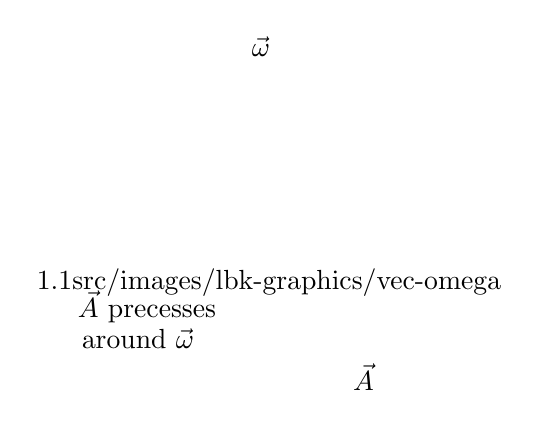
\begin{tikzpicture}
%   \draw[help lines,step=.5,lightgray] (-3,-3) grid (3,3) ;
%     \foreach \y in {-3,-2.5,...,3}
%     \draw (-3.2,\y) node[left]{\tiny\y} ;
%     \foreach \x in {-3,-2.5,...,3}
%     \draw (\x,3.2) node[above]{\tiny\x} ;
  \node at (0,0) 
{\ingr{1.1}{src/images/lbk-graphics/vec-omega}};
  \node at (-.1,3) {$\vec{\omega}$} ;
  \node at (-2.55,-.3)[right] {$\vec{A}$ precesses} ;  
  \node at (-2.5,-.7)[right]  {around $\vec{\omega}$} ; 
  \node at (1.2,-.9) [below]{$\vec{A}$} ;
  \node at (0.2,-1.6) {$\gkq$} ;
 \end{tikzpicture}
 \caption{}\label{fig2.2}
\end{figure}

\hbf{The meaning of the vector {$\vec{\omega}$}{}}

Observe that a vector $\vec{A}$ which is {at rest} relative 
to $S^\bst$ has $\dd ^{\bst}\vec{A}/\dd t = 0 $ and  
hence 
\eqref{nif.7} reduces to
\begin{align}\label{nif.8}
 \dv{A}{t} = \,\vec{\gkw}\times \vec{A}.
\end{align}
This is a differential equation expressed relative to the  
Galilei frame $S$ and we shall interpret it by appealing to 
its general solution. First, we consider the case when 
$\,\vec{\gkw}$ is a constant. Then, dot multiplying 
\eqref{nif.8} by $ \,\vec{\gkw}$, we get, as  
$\,\vec{\gkw}$ is a constant,
\begin{align*}
\dv{}{t} (\,\vec{\gkw}\dotp \vec{A})=0,
\end{align*}
which shows that the the projection of $\vec{A}$ on to 
$\,\vec{\gkw}$ is a constant of motion. Next, 
dot-multiplying Eq.\eqref{nif.8} by $\vec{A}$, we get
\begin{align*}
\dv{}{t} (\vec{A}\dotp \vec{A})=0,
\end{align*}
which implies that $|\vec{A}|$ is another constant of 
motion.

Thus, $\vec{A}$ moves such that it makes a constant 
angle with $\,\vec{\gkw}$ while keeping its length 
constant. To determine the orbit of the tip of 
$\vec{A}$ explicitly, we choose the $z$-axis (of $S$) 
along the constant vector $\,\vec{\gkw}$ so that 
$\,\vec{\gkw} =\gkw \kay$. Then the equations of motion 
in Eqn.\eqref{nif.8} are 
\begin{align}\label{nif.8a}
\dotup{A}_x =-\gkw A_y,\quad 
\dotup{A}_y =\gkw A_x, \quad \dotup{A}_z =0. 
\end{align} 
Introducing the complex variable $\xi \equiv A_x +i A_y $, 
we combine the first two equations into the single equation
\begin{align*}
\dotup{\xi} =i \gkw(A_x +iA_y)=i\gkw
\xi,\quad \dotup{\xi}\equiv
(\dd \xi/\dd t).
\end{align*}
This equation has the general solution
\begin{align*}
\xi =\xi(0)\, e^{i \gkw t}.
\end{align*}
which clearly shows that, $\xi$, or, what is the same 
thing, $\vec{A_{\perp}} =\eye A_x +\jay A_y$, the 
projection of $\vec{A}$ on to the $x-y$ plane, rotates 
with the constant angular speed $\gkw$. Since  
$\dotup{A}_z =0$ (see Eqn.\eqref{nif.8a}), it follows 
that  $\vec{A}_\shortparallel=\kay A_z$ is a constant . 
This implies that the vector 
$\vec{A}=\vec{A}_\shortparallel +\vec{A}_{\perp}$,  
with its initial point $O$ fixed, moves over a 
(right-circular) cone whose axis along $\kay $ or, 
$\hat{\gkw}$, as shown in \figref{fig2.2}.  Such a 
motion is called a \textsl{precession} about the 
(constant) vector $\,\vec{\gkw}$.

Clearly, the above conclusions are independent of the 
value of the (constant) angle $\gkq$ and the (constant) 
length $|\vec{A}|$. If we notice that $\vec{A}$, 
geometrically, is the position vector 
$x^{\bst}\eye^{\bst}+ y^{\bst}\jay^{\bst}+ 
z^{\bst}\kay^{\bst}$ of a fixed  point of the frame 
$S^\bst$, we conclude that the rigid frame $S^\bst$ 
itself executes a precessing motion about the vector 
$\,\vec{\gkw}$. Thus, \textsl{the vector $\,\vec{\gkw}$ 
in Eqn.\eqref{nif.8} is the (constant) angular 
velocity} of the rigid frame $S^\bst$ relative to the 
Galilei frame $S$.

\hsl{Meaning of $\,\vec{\gkw}$ when it is a 
function of time} Consider $\,\vec{\gkw}(t)$ at a frozen 
instant of time, say, $t=t_0$ and observe that 
$\,\vec{\gkw}(t_0)$ is the angular velocity of $S^\bst$ 
relative to $S$.  Therefore, \textsl{the non-constant 
vector$\,\vec{\gkw}(t)$ is the instantaneous angular 
velocity} of the rotating Cartesian coordinate system 
$S^{\bst}$ relative to the Galilei frame 
$S$.\vspace{1\bsk}

\hsl{Note 1}Before passing, we may recall that 
according to Eqn.\eqref{nif.7}, the time-derivatives of 
a vector function in the two frames would be equal if 
the two frames do not rotate relative to one another, 
i.e., if $\vec{\gkw}=0$. The advancing frame discussed 
in \S~2.6 is a typical example. \vspace{1\bsk}

\hsl{Note 2}More, importantly, when $S^\bst$ is 
obtained from (the absolute frame) $S$ by a Galilei 
transformation, then also $\vec{\gkw}=0$ and the 
time-derivatives of a vector function in the two frames 
are equal. This would mean that the time-derivative of 
a vector function would be the same in all Galilei 
frames so that we can use a common notation for it, 
namely $\bdv{\vec{A}}{t}$ as done earlier in this 
section. 

\vspace{-.3cm}

\section{Transformation of velocity}
\index{transformation ! of velocity} Using the formula 
\eqref{nif.7}, we may obtain the transformation laws 
for  the velocity and acceleration of a point particle 
under a change from the Galilei frame $S$ to a general 
accelerated frame $S^\bst$. Recall that a {general 
accelerated frame} $S^\bst$ has the most general 
rigid-body motion relative to the Galilei frame $S:\{O, 
\eye, \jay, \kay \}$.

Let $\vec{r}=\vec{OP}$ and $\vec{r}^{\,\bst} 
=\vec{O^\bst P}$ be the position vectors of a point 
particle $P$ relative to $S$ and $S^\bst$ at the 
(absolute) time $t$. Then, as shown in \figref{fig2.3}, 
the positions $\vec{r}$ and $\vec{r}^{\,\bst}$ of $P$ 
are related by
\begin{figure}[H]
\begin{center}
\begin{tikzpicture}
%  \draw[help lines,step=.5,lightgray] (-3,-3) grid (3,3);
%     \foreach \y in {-3,-2.5,...,3}
%     \draw (-3.2,\y) node[left]{\tiny\y} ;
%     \foreach \x in {-3,-2.5,...,3}
%     \draw (\x,3.2) node[above]{\tiny\x} ;
\node at (0,0)%
{\ingr{.5}{src/images/lbk-graphics/Diagram2a.pdf}} ;
  \node at (-2.25,-1.2) {\small $O$} ;
  \node at (1.85,-1.1) {\small $O^\bst$} ;
  \node at (2.2,1.35) {\small $P$} ;
  \node at (-.35,0) [left]{ $\vec{r}$} ;
  \node at (2.2,0) {$\svec{r}$} ;
  \node at (0,-1.5){$\vec{R}$} ;
  \end{tikzpicture}
  \caption{}  \label{fig2.3}
\end{center}
\end{figure}
\begin{align}\label{nif.9}
\vec{r} = \vec{R}+\vec{r}^{\,\bst }, \quad
\vec{R}\equiv \vec{OO^{\bst}},
\end{align}
where we have used the Euclidean law of addition of 
vectors. The Galilei frame-time-derivative of $\vec{r}$ 
is then given by,
\begin{align}\label{nif.10}
 \dv{\vec{r}}{t} = \dv{\vec{R}}{t} +  
\dv{\vec{r}^{\,\bst}}{t}.
\end{align}
The second term on the right hand side above is a hybrid 
term: It is the $S$-frame derivative of a $S^\bst$-frame 
vector and it has no obvious meaning. To get round this 
difficulty, we replace the Galilei frame-operator 
$\dd /\dd t$ by $(\dd^{\bst} /\dd t  
+\,\vec{\gkw}\times)$ 
using Eqn.\eqref{nif.7} and obtain
\begin{align}\label{nif.11}
\dv{\vec{r}}{t} = \dv{\vec{R}}{t}
+\left(\frac{\dd^{\bst}}{\hspneg\dd t}
+\,\vec{\gkw}\times\right)\svec{r}.
\end{align}
Here, we observe that
\begin{align}\label{nif.12}
\vec{u}&=\dv{\vec{r}}{t}, \notag
\intertext{and} 
\svec{u}& =\ldv{\bst}{\svec{r}}{t},
\end{align}
are the velocities of the particle $P$ relative to $S$ and
$S^{\bst}$ respectively, and
\begin{align}\label{nif.13}
\vec{v}\equiv \dv{\vec{R}}{t},
\end{align}
is the velocity of $O^{\bst}$ relative to $O$ (or, what 
is the same thing, the (linear) velocity of $S ^{\bst}$ 
relative to $S$ ). Thus, Eqn.\eqref{nif.11} may be 
written as
\begin{align}\label{nif.14}
\vec{u} = \vec{v} 
+(\,\vec{\gkw}\times\vec{r}^{\,\bst})+ \svec{u},
\end{align} 
which is the required formula {relating the 
velocity $\vec{u}$ of a particle in a Galilei frame 
with its velocity $\vec{u}^\bst$ in a general 
accelerated (Cartesian) frame}. If the particle $P$ is 
permanently at rest in $S^\bst$, its velocity relative 
to $S^\bst$ would be zero, but it would still have a 
non-zero velocity in the Galilei frame given by
\begin{align}\label{nif.15}
\vec{u} \equiv \vec{u}_t= \vec{v} +
(\,\vec{\gkw}\times\svec{r}) .
\end{align}
The velocity $\vec{u}_{_T}$, of a particle $P$ which is 
permanently at rest in $S^\bst$, is called the 
\textsl{velocity of transport} as it arises due to the 
transport of the particle by the moving frame as seen 
from the Galilei frame. Using Eqn.\eqref{nif.15} in 
Eqn.\eqref{nif.14}, we may express the latter as
\begin{align}\label{nif.14a}
\vec{u} = \vec{u}_t + \svec{u}.
\end{align}
\section{Coriolis acceleration}
\index{Coriolis Theorem}
\index{transformation ! of acceleration}
Differentiating Eqn.\eqref{nif.14} once more with 
respect  to absolute time $t$, we get
\begin{align}\label{nif.18}
\dv{\vec{u}}{t}&= \dv{\vec{v}}{t} +
\dv{\,\vec{\gkw}}{t}\times\svec{r}
+\,\vec{\gkw}\times\dv{\svec{r}}{t}
+ \dv{\svec{u}}{t}\notag \\
& =\dv{\vec{v}}{t} +(\dv{\,\vec{\gkw}}{t}\times
\vec{r}^{\,\bst } )
+\,\vec{\gkw}\times\left( \dv{^{\bst}}{t}
+\,\vec{\gkw} \times\right) \vec{r}^{\,\bst }\notag\\
& \qquad+\left( \dv{^{\bst}}{t}
+\,\vec{\gkw} \times\right) \svec{u},
\end{align}
where we have replaced the operator $\dd/ \dd t$ by  
$(\dd^{\bst}/\dd t +\vec{\gkw} \times)$ using 
Eqn.\eqref{nif.7}. Rearranging, we obtain

\begin{align}
\dv{\vec{u}}{t}&=
\dv{\vec{v}}{t} \, + \dv{\,\vec{\gkw}}{t}\times \svec{r}
 +\vec{\gkw} \times\svec{u}+  
\,\vec{\gkw}\times(\vec{\gkw}\times \svec{r})\notag \\
&\qquad \qquad  +\dv{^{\bst}\svec{u}}{t}
+ \vec{\gkw} \times \svec{u} \notag \\
& = \dv{\vec{v}}{t}
+\dv{\,\vec{\gkw}}{t}\times \svec{r} +
\,\vec{\gkw}\times (\vec{\gkw} \times \svec{r})
+2 \vec{\gkw}\times\svec{u}\notag \\
&\qquad \qquad +\dv{^{\bst}\svec{u}}{t}.
\end{align}
In this equation, we readily identify 
\begin{align}\label{nif.19} 
\vec{a}\equiv \dv{\vec{u}}{t},
\end{align}
as the acceleration of the particle $P$ relative to the 
Galilei frame $S$,
\begin{align}\label{nif.20}
\svec{a} \equiv
\dv{^{\bst}\svec{u}}{t},
\end{align}
as the acceleration of $P$ relative to $S^\bst$, and 
\begin{align}\label{nif.21} \vec{\alpha}\equiv 
\dv{\vec{v}}{t},
\end{align}
as the (linear) acceleration of $S^\bst$ relative to 
$S$. Further, we  introduce the notation\footnote{Note 
the interesting relation $(\dd \,\vec{\gkw}/\dd t)= 
(\dd ^{\bst }\vec{\gkw}/\dd t)$, which follows from 
Eqn.\eqref{nif.7} when we take $\vec{A}=\vec{\gkw}$. 
This relation implies that $\vec{\gkw}(t)$ has the same 
time-development relative to both the frames $S$ and 
$S^\bst$. As such, we may use a common notation 
$\dotup{\,\vec{\gkw}}$ for the 
time-derivative of $\vec{\gkw}(t)$.}
\begin{align}\label{nif.22}
 \dot{\,\vec{\gkw}}\equiv
\dv{\,\vec{\gkw}}{t}=
\dv{^{\bst}\vec{\gkw}}{t},
\end{align}
and rewrite the equation Eqn.\eqref{nif.18} as
\begin{align}\label{nif.23}
\vec{a}& =\Big\{ \vec{\alpha} +(\dotup{\,\vec{\gkw}}
\times \svec{r}) + \,\vec{\gkw}\times ( \,\vec{\gkw} 
\times \svec{r} )\Big \}\notag\\&\qquad+
2(\,\vec{\gkw}\times\svec{u}) +\svec{a}.
\end{align}
This formula relates the accelerations $\vec{a}$ and 
$\svec{a}$ of a point particle $P$ in the two Cartesian 
coordinate systems $S$ and $S^\bst$. It is important to 
note that under the transition from the Galilei frame 
$S$ to an accelerated frame $S^\bst$, $\vec{a}\neq 
\svec{a}$, unlike in the case of a Galilei 
transformation.

In particular, if $P$ is fixed in $S^\bst$, that is, if 
$\svec{u}$ is constantly zero in $S^\bst$, then $P$ 
would have the acceleration $\vec{a}=\vec{a}_{\sfx{t}}$ 
relative to the Galilei frame $S $ where
\begin{align}\label{nif.24}
\vec{a}_{\sfx{t}}\equiv\vec{\alpha}
+(\dotup{\,\vec{\gkw}}\times \svec{r}) +
\,\vec{\gkw}\times \big( \,\vec{\gkw} \times
\vec{r}^{\,\bst} \big ).
\end{align}
The acceleration $\vec{a}_{\sfx{t}}$ is called the 
\textsl{acceleration of transport}. The term
\begin{align}\label{nif.25}
\vec{a}_{c}\equiv2(\,\vec{\gkw}\times\svec{u}),
\end{align}
is called the \textsl{Coriolis 
acceleration}\footnote{Unlike 
what we have done above, some authors, including Banach, 
loc.cit., p.61, call $-2 \,\vec{\gkw}\times\svec{u}$ as the 
Coriolis acceleration.} after its discoverer G. Coriolis. 
Thus, we may rewriteEqn.\eqref{nif.23} compactly as
\begin{align}\label{nif.26}
\vec{a}=\svec{a}+\vec{a}_{\sfx{t}}
+\vec{a}_{\sfx{c}}.
\end{align}
The Coriolis acceleration is an important parameter in 
engineering kinematics and in long-range 
ballistics\footnote{D. E. Christie, 1964, 
\textsl{Vector Mechanics}, Second Edition, McGraw-Hill 
Book Company, New York, \S~14.4.}. We note that the 
Coriolis acceleration is zero when there is no rotation 
($\vec{\gkw}=0$), if the relative velocity $\svec{u}$ 
is parallel to $\vec{\gkw}$, or, if $\svec{u}=0$.

In passing, we note that the frame $S^\bst$ is 
specified completely by giving the new Cartesian 
coordinates $x^{\bst}, y^{\bst},z^{\bst}$ as functions 
of the Cartesian coordinates $x,y,z$ in the Galilei 
frame $S$ and the (absolute) time parameter $t$. 
However, many a times it would be sufficient to specify 
$S^\bst$ \textsl{partially} by giving the pairs of 
vector parameters $\{\vec{R},\,\vec{\gkw}\}$, or 
$\{\vec{v},\,\vec{\gkw}\}$ or $\{\vec{A},\, 
\vec{\gkw}\}$.

\section{Dynamics in an accelerated frame} Note that  
in the discussion of the previous section the frame 
$S$ has been chosen to be a Galilei frame and the 
other, $S^\bst$, is chosen to be an a Cartesian 
coordinate system in arbitrary rigid body motion 
relative to $S$. In any such discussion, it is 
customary to call the Galilei frame $S$ as the 
``absolute frame'' and $S^\bst$ shortly as an 
accelerated frame. However, we remind the reader that 
the name ``absolute frame'' $S$ in such discussions 
would refer to any one of the Galilei frames and not 
the absolute frame of Newton !

Suppose a particle $P$ of mass $m$ moves under the 
action of a force (also called physical or applied 
force)            $\vec{F}_{\sfx{a}}$ in the Galilei 
frame $S$. (The suffix $a$ in $\vec{F}_{\sfx{a}}$ 
derives from the Newtonian nomenclature ``absolute 
force''.) Then, according to the second law of Newton, 
we have
\begin{align}\label{nif.27}
m\vec{a}=\vec{F}_{\sfx{a}}.
\end{align}
Using the acceleration-transformation formula 
\eqref{nif.26}, we
rewrite Eqn.\eqref{nif.27} as
\begin{align}\label{nif.28}
m(\svec{a}+\vec{a}_{\sfx{t}} + \vec{a}_{\sfx{c}}
)=\vec{F_{\sfx{a}}},
\end{align}
and rearrange it as
\begin{align}\label{nif.29}
m\svec{a}=\vec{F_{\sfx{a}}}-m\vec{a}_{\sfx{t}}
-m\vec{a}_{\sfx{c}}.
\end{align}
Now, we define two \textsl{force-like terms}:
\begin{align}\label{nif.30}
\vec{F}_{t}& \equiv -m\vec{a}_{\sfx{t}}\notag\\&
=-m\vec{\alpha}
-m\dotup{\,\vec{\gkw}}\times \vec{r}^{\,\bst }
-m\,\vec{\gkw}\times ( \,\vec{\gkw} \times 
\vec{r}^{\,\bst}),
\end{align}
called the \textsl{fictitious force of transport}, and
\begin{align}\label{nif.31}
\vec{F}_{c} \equiv -m \vec{a}_{\sfx{c}}
=-2m\,\vec{\gkw}\times\svec{u},
\end{align}
called the \textsl{fictitious force of Coriolis}. Then, the 
equation of motion of a particle in the frame $S^\bst$, 
i.e., Eqn.\eqref{nif.29}, takes the form
\begin{align}\label{nif.37x}
m\svec{a}=\vec{F_{\sfx{a}}}+\vec{F}_{\sfx{t}}
+\vec{F}_{\sfx{c}}.
\end{align}
If we define a `force' $\vec{F}^\bst$ by 
$\vec{F}^\bst\equiv 
\vec{F_{\sfx{a}}}+\vec{F}_{\sfx{t}}  
+\vec{F}_{\sfx{c}}$, 
this equation of motion in the accelerated frame $S^\bst$ 
becomes
\begin{align}
m\svec{a}=\vec{F}^\bst,
\end{align}
which \textsl{formally resembles} the Newton's second 
law of motion.  Moreover, then, the Newton second law 
of motion would be true relative to an accelerated 
frame also ! However, this resemblance is purely formal 
because $\vec{F}_{t}$ and $\vec{F}_{c}$ are two 
``force-like terms'' (i.e., terms having the physical 
dimensions of a force) and not `true' (or, 
physically-applied) forces unlike $\vec{F_{\sfx{a}}}$. 
We may appreciate using the phrase ``force-like terms'' 
 better if we recall that an applied force such as 
$\vec{F}_{\sfx{a}}$ is by definition an absolute vector 
quantity (in the Newtonian regime) and would therefore 
be the \textsl{same} (vector) in all accelerated 
coordinate systems $S^\bst$. In sharp contrast, 
\textsl{the fictitious forces $\vec{F}_{t}$ and 
$\vec{F}_{c}$ are not absolute quantities} and in 
general, \textsl{they vary from one accelerated frame 
to another.} 
\begin{align*}
& \pvec{F}_{\sfx{t}}=-m\pvec{\alpha}
-m\dotup{\vec{\gkw}'} \times \pvec{r} -m
\,\pvec{\gkw}\times ( \,\pvec{\gkw}\times \pvec{r}),\\
& \pvec{F}_{\sfx{c}}  
=-2m\,\pvec{\gkw}\times\pvec{u},
\end{align*}
where $\pvec{\alpha}$, $\pvec{\gkw}$, $\pvec{r}$, and
$\pvec{u}$ have their usual meaning relative to $S^\bst$.
\section{An advancing frame}
\index{accelerated frame ! advancing}
Consider the coordinate transformation
\begin{align}\label{gt.4}
&\svec{r}= \vec{r}-\vec{g}(t),\;\vec{g}(t)\equiv
g(t)\,\hat{g},\;
\hat{g}=\text{constant},\notag \\
&\eye^\bst=\eye,\; \jay^\bst=\jay,\;\kay^\bst=\kay,
\end{align}
from the Galilei frame $S:\{x,y,z\}$ to a new Cartesian 
coordinate system $S^\bst:\{x^\bst,y^\bst,z^\bst\}$. We 
assume that $g(t)$ in Eqn.\eqref{gt.4} is any arbitrary 
vector function of $t$. Below, we will show that the frame 
$S^\bst$ so obtained has an advancing motion with a 
{non-constant} acceleration $\vec{g}(t)$ relative to the 
Galilei frame $S$.

Comparing Eqn.\eqref{gt.4} with the generic 
transformation\break Eqn.\eqref{nif.9}, we note that 
$\vec{R}(t)=-\vec{g}(t)$ here. Also, we observe that 
the transformation Eqn.\eqref{gt.4} leaves the base 
vectors unchanged which implies that the Cartesian 
coordinate system $ S^\bst$ remains parallel to $S$ (at 
all times). In other words, there is no rotation 
involved in the transformation Eqn.\eqref{gt.4} so that 
$\vec{\gkw}=0$. Then, the generic velocity 
transformation rule Eqn.\eqref{nif.14} gives 
\begin{align}
\vec{u}= \svec{u}+\vec{v}=\svec{u}
+\dot{\vec{R}}(t)=\svec{u}-\dot{\vec{g}}(t).
\end{align}
Similarly, the generic acceleration transformation rule  
Eqn.\eqref{nif.23} gives 
\begin{align} 
\vec{a}&= \vec{\alpha}+\svec{a}=\dv{\vec{v}}{\dd 
t}+\svec{a} 
=\ddot{\vec{R}}(t)+\svec{a}=-\ddot{\vec{g}}(t) 
+\svec{a}. 
\end{align} 
Thus, the accelerations of a point particle in the two 
frames are related by
\begin{align}\label{nif.40}
\svec{a}=\vec{a}+\ddot{\vec{g}}(t),
\end{align}
In particular, if $\vec{a}=0$, which is true of a 
point-particle which is free of forces in the Galilei 
frame $S$, then $\svec{a}=\ddot{\vec{g}}(t)$. Thus {a 
free-particle moves with an acceleration 
$\svec{a}=\ddot{\vec{g}}(t)$ 
relative to the accelerated frame}$S^\bst$. (This 
observation shows again that the first law of Newton is not 
valid in the accelerated frame $S^\bst$.) Finally, we 
consider a general {reference point} of the accelerated 
frame $S^\bst$ which is simply a spatial point with fixed 
(=constant in time) but arbitrary spatial coordinates 
$(x^\bst,\,y^\bst,\,z^\bst)$. Clearly, every reference 
point of the accelerated frame $S^\bst$ has zero 
acceleration ($\svec{a}=0$), and using this information 
in Eqn.\eqref{nif.40}, we obtain
\begin{align}
\vec{a}=-\ddot{\vec{g}}(t),
\end{align}
which is the (Galilei)$S$-frame acceleration of a
{general reference point} of the accelerated frame
$S^\bst$. Hence the frame $S^\bst$ itself moves with the
acceleration $-\ddot{\vec{g}}(t)$ relative to $S$. The
assumed constancy of the direction of the vector $\vec{g}$
implies that the motion $S^\bst$ relative to $S$ is a pure
advancing motion.

\vspace{-.3cm}

\section{A frame attached to a rotating  turn-table}
\index{rotating turn-table} 
Let $S$ be a Galilei frame and $S^\bst$ be the frame 
attached to the rotating turn-table. We specify the motion 
of $ S^\bst$ relative to $S$ by giving a transformation 
connecting the base vectors of the two frames:
\begin{align}\label{nif.42}
\begin{pmatrix}
\eye^{\bst}\\ \jay^{\bst}\\ \kay^{\bst}
\end{pmatrix}
=\begin{pmatrix}
c & s & 0\\
-s & c& 0 \\
0\;\;&0&1\end{pmatrix} \begin{pmatrix}\eye\\
\jay\\\kay\end{pmatrix}
\end{align}

\newpage

\begin{figure}[H] 
\begin{center}
\begin{tikzpicture}
%   \draw[help lines,step=.25,brown] (-5,-5) grid (5,5) ;
%   \foreach \y in {-4.5,-4,...,4.5,}
%     \draw (-5.2,\y) node[left]{\small \y} ;
%     \foreach \y in {-5,-4.5,...,4,4.5}
%     \draw (5.2,\y) node[right]{\small \y} ;  
%   \foreach \x in {-4.5,-4,...,5}
%     \draw (\x,5.15) node{\small \x} ;
%       \foreach \x in {-5,-4,...,5}
%     \draw (\x,-5) node[below]{\small \x} ;
\node at (0,0){\ingr{1}{src/images/lbk-graphics/turn-table.pdf}};
\node at (-.25,-.25){\small  $\gkf$} ;
\node at (1.45,1){\small  $\suvec{\imath}$} ;
\node at  (-2.15,1){\small  $\suvec{\jmath}$} ;
\node at (-1.2,-2.5){\small  $\uvec{k}=\suvec{k}$} ;
\node at (2.7,-.75) {\small  $\uvec{\imath}$} ;
\node at (-.5,2.5){\small  $\uvec{\jmath}$} ;
\end{tikzpicture}
\caption{A frame attached to a rotating 
turn-table}\label{fig2.4}
\end{center}
\vspace{-.5cm}
\end{figure}
where $c\equiv \cos \phi$, $s\equiv \sin \phi$ and 
$\phi$ is some differentiable function of time where we 
have assumed, for simplicity, that the origins $O$ and 
$O^{\bst}$ of the two frames coincide and the 
turn-table rotates about the common $\kay-\kay^{\bst}$ 
axis as shown in \figref{fig2.4}.
The inverse basis transformation is given by
\begin{align}\label{nif.39}
\begin{pmatrix}\eye\\ \jay\\\kay\end{pmatrix}
=\begin{pmatrix} c & - s & 0\\
c & s& 0 \\
0\;\;&0&1\end{pmatrix} \begin{pmatrix}\eye^{\,\bst}\\
\jay^{\,\bst}\\\kay^{\,\bst}\end{pmatrix} .
\end{align}
Then, with $\dotup{\phi}\equiv \gkw $ denoting $
\dd \phi/\dd t $, we have, on using Eqn.\eqref{nif.42},
\begin{align}\label{nif.39a}
&\dd \eye^{\bst}/\dd t =\dotup{\phi}
\left(-s \,\eye+c \,\jay\right), \notag \\
&\dd \jay^{\bst}/\dd t =\dotup{\phi}\left(
-c\,\eye-s\, \jay\right), \notag \\
&\dd \kay^{\bst}/\dd t =0,
\end{align}
so that, from Eqn.\eqref{nif.5}--\eqref{nif.5b} and 
\eqref{nif.6}, we get the angular velocity of $S ^{\bst}$ 
relative to $S$ :
\begin{align}
\vec{\gkw}&= \eye^{\bst}\left(\dv{ \jay^{\bst}}{t}
\dotp\kay^{\bst}\right)
+\jay^{\bst}\left( \dv{\kay^{\bst}}{t}
\dotp\eye^{\bst}\right)
+\kay^{\bst}\left( \dv{\eye^{\bst}}{t}
\dotp\jay^{\bst}\right)\notag \\
&=\kay^{\bst}\left(\dotup{\phi}(-s \,\eye+c \, \jay) 
\dotp(-s \eye +c \jay)\right) 
=\dotup{\phi}\,\kay^{\bst}=\dotup{\phi}\, \kay. 
\end{align}
where we have used the property that 
$\kay^{\bst}=\kay$ is a constant vector under the 
transformation \eqref{nif.42}. Finally, differentiating 
the above expression for $\vec{\gkw}$, we get the 
angular acceleration
\begin{align}
\dotup{\vec{\gkw}}&= \ddotup{\phi}\,\kay^{\bst}
=\ddotup{\phi}\, \kay.
\end{align}
\subsection{Motion relative to  a uniformly
rotating  frame}
\index{frame ! uniformly rotating }
If $S$ is a Galilei frame, then a Cartesian coordinate 
system $S^\bst$ which has a pure, uniform, rotating 
motion relative to $S$ has, by definition 
$\vec{\alpha}=0 $ and $\,\vec{\gkw}=$ constant, say 
$\,\vec{\gkw}_0 $. If we choose the constant vector 
$\,\vec{\gkw}_0$ conveniently along the 
$\kay^{\bst}$-axis of $S^\bst$, we have $\,\vec{\gkw}_0 
=\gkw_0 \kay^{\bst}$. Then, the fictitious forces in 
$S^\bst$ are \begin{align}\label{nif.35} \vec{F}_{t} \equiv 
\vec{F}_{\sfx{CF}}= -m \,\vec{\gkw}_0\times ( 
\,\vec{\gkw}_0 
\times \vec{r}^{\,\bst }),
\end{align}
called the \textsl{centrifugal fictitious force}, and
\begin{align}\label{nif.36}
\vec{F}_{c}=-2m\,\vec{\gkw}_0\times\svec{u}.
\end{align}
which is the Coriolis force. Resolving $\vec{r}^{\,\bst }$ 
into sum of a vector $\vec{r}_{\parallel}^{\,\bst }$ along 
$\,\vec{\gkw}_0$ and a vector $\vec{\rho}$ perpendicular to 
$\,\vec{\gkw}_0 $, we rewrite the centrifugal fictitious 
force as
\begin{align}\label{nif.37}
\vec{F}_{\sfx{CF}} &=-m \,\vec{\gkw}_0
\times [\,\vec{\gkw}_0\times
\{\vec{r}_{\parallel}^{\,\bst } +\vec{\rho}\} ]
 \notag\\&= -m \,\vec{\gkw}_0 \times [ \,\vec{\gkw}_0
\times \vec{\rho} ]\notag\\&
= -m\,\vec{\gkw}_0 (\,\vec{\gkw}_0 \dotp
\vec{\rho}) + m\vec{\rho}
(\,\vec{\gkw}_0 \dotp \,\vec{\gkw}_0) \notag\\&
= m\gkw_0^2 \vec{\rho}.
\end{align}
This familiar form of the centrifugal 
'pseudo-force-field' which exists in $S^\bst$ shows 
that it is perpendicular to the axis of rotation 
$\hat{\gkw}_0$, increases linearly with the 
perpendicular distance $\rho$ and acts in the direction 
$ \hat{\rho}$ which is radially away from the axis 
$\hat{\gkw}_0$.

\exm Consider a free particle $P$ which is at rest in the
Galilei frame $S$. Discuss its motion relative to an 
accelerated frame $S^\bst$ which rotates uniformly with the 
angular velocity $\vec{\gkw}$ relative to $S$. Assume that 
$S^\bst$ has no translatory motion with respect to $S$ and 
the $\kay-\kay^\bst$ axes of the two frames coincide.

\soln Evidently, this problem concerns motion relative to a 
uniformly rotating frame. We are given $F_a=0$ as $P$ is 
given to be free in the Galilei frame $S$., Therefore, its 
equation of motion Eqn.\eqref{nif.37x} in $S^\bst$ is (cf. 
\S~2.7.1)
\begin{align}
m\svec{a}&=\vec{F}_\sfx{CF} +\vec{F}_{\sfx{c}}\notag\\
&=-m \,\vec{\gkw}_0\times ( \,\vec{\gkw}_0 \times
\vec{r}^{\,\bst})-2m\,\vec{\gkw}_0\times\svec{u} .
\end{align}
Using the relation Eqn.\eqref{nif.14} in which, now, 
$\vec{u}=0$ 
(particle $P$ is at rest in $S$) and $\vec{v}=0$ (the frame 
$S^\bst$ has no translatory motion relative to $S$), for 
$\svec{u}$, we may rewrite the last term as,
\begin{align}\label{2.53x}
m\svec{a}&=-m \,\vec{\gkw}_0\times ( \,\vec{\gkw}_0 \times
\vec{r}^{\,\bst})
+2m\,\vec{\gkw}_0\cross(\vec{\gkw}\cross\svec{r})\notag\\
&=m\,\vec{\gkw}_0\cross(\vec{\gkw}\cross\svec{r})
=-m\gkw_0^2 \vec{\rho},
\end{align}
where, as we did in Eqn.\eqref{nif.37}, we have resolved 
$\vec{r}^{\,\bst}$ into sum of a vector 
$\vec{r}_{\parallel}^{\,\bst }$ along $\,\vec{\gkw}_0$ and 
a 
vector $\vec{\rho}$ perpendicular to $\,\vec{\gkw}_0 $. 
Clearly Eqn.\eqref{2.53x} represents \textsl{circular 
motion} under the \textsl{centripetal} force $-m\gkw_0^2$ 
about $\vec{\rho}=0$ in a plane perpendicular to 
$\,\vec{\gkw}_0 $. This describes the familiar situation 
that 
for some body who spins uniformly about a vertical axis 
with 
the constant angular velocity $\vec{\gkw}$, everything (at 
rest) around appears to move round in circles with the 
opposite angular velocity.

\exm Express the basis-vector-transformation  
Eqn.~\break\eqref{nif.42} as a coordinate transformation 
connecting 
the two frames $S$ and $S^\bst$. 

% Since the particle $P$ is 
% free, its $S$-frame acceleration is zero.

\soln First, a note on matrix notation that we employ here: 
We use the overhead `tilde' $\sim$ to denote matrix  
transpose: $\tilde{X}$ is the transpose of the column 
matrix 
$X$. Also, the asterisk $\bst$ should not be misunderstood 
to indicate complex conjugation; here, it simply marks the 
variable as one belonging to the frame $S^\bst$. as
\begin{align}\label{af.42}
& X^\bst=\mathsf{R}\,X,\quad
\tilde{X}^\bst=(x^\bst y^\bst
z^\bst),\quad \tilde{X}
=(x y z),\notag \\
& \mathsf{R}=\begin{pmatrix}\cos\,\gkq&-\sin\,
\gkq&0\\\sin\,\gkq&\cos\,\gkq
&0\\0&0&1\end{pmatrix} ,\quad
\gkq=\gkq(t).
\end{align}

We recall the following result from the theory of linear 
spaces: In a $n$-dimensional linear space $V_n\ni \vec{0}, 
\, 
\vec{x}, \,\vec{y},\,\vec{z},$, let $\{\vec{b}_i\}$, 
$i=1,2,3,\dots,n$ be a basis and
\begin{align}\label{base}
 \vec{x}=\sum_{i=1}^n x^i\vec{b}_i,
\end{align}
be the expansion of a vector $\vec{x}\in V_n$ in this 
basis. Defining a column matrix of basis vectors
\begin{align}
\mathcal{B}=\begin{pmatrix}
\vec{b}_1\\\vec{b}_2\\ \vdots\\\vec{b}_n
\end{pmatrix},
\end{align}
also called a \textsl{stack} of basis vectors, or a 
\textsl{basis-stack}, we may express Eqn.\eqref{base} in 
matrix form as follows:
\begin{align}
 \vec{x}=\sum_i^n x^i\vec{b}_i=\tilde{\mathcal{B}}X,
\end{align}
Also, a basis change such as
\begin{align}\vec{b}_i\mapsto\svec{b}_i \equiv \sum_j
\mtud{T}{j}{i}\vec{b}_j,
\end{align}
where $\mtud{T}{j}{i}$, $i,\,j=1,\,2,\,\dots,n$ are $n^2$ 
scalars from the  ground field of $V_n$, may be expressed 
in matrix notation as
\begin{align}
\mathcal{B}^\bst=\mathsf{T}\mathcal{B},
\end{align}
where
\begin{align}
\mathcal{B}^\bst\equiv \begin{pmatrix}
\svec{b}_1\\\svec{b}_2\\ \vdots\\\svec{b}_n\end{pmatrix},\;
\mathsf{T}\equiv \begin{pmatrix}
\mtud{T}{1}{1}& \mtud{T}{2}{1}&\dots & \mtud{T}{n}{1}\\
\mtud{T}{1}{2}& \mtud{T}{2}{2}&\dots & \mtud{T}{n}{2}\\
&.&\dots &.\\
\mtud{T}{n}{2}& \mtud{T}{n}{2}&\dots & 
\mtud{T}{n}{2}\\;
\end{pmatrix},\quad\det{\mathsf{T}}\neq 0.
\end{align}
Now, it is a well known 
result from the theory of linear spaces that the column 
matrices
\begin{align}\label{af.47}
 \mathsf{X}=\begin{pmatrix}
x^1\\x^2\\ \vdots\\x^n
\end{pmatrix}, \quad \mathsf{X}^\bst=\begin{pmatrix}
x^{\bst 1}\\x^{\bst 2}\\ \vdots\\x^{\bst n}
\end{pmatrix},
\end{align}
of the vector components of a vector $\vec{x}\in V_n$, in 
the 
two bases $\mathcal{B}$ and $\mathcal{B}^\bst$ connected by 
\eqref{af.47}, are related by
 \begin{align}
\mathsf{X}^\bst=
\tilde{\mathsf{T}}^{-1}\mathsf{X}.
 \end{align}

In the light of the above result, we observe that the basis 
transformation Eqn.\eqref{nif.42} may be written, more 
explicitly, as
\begin{align}\label{gt.6}
\mathcal{B}^\bst&\equiv 
\begin{pmatrix}\eye^\bst\\\jay^\bst\\
\kay^\bst\end{pmatrix}
=\tilde{\mathsf{R}}^{-1}\mathcal{B}
=\begin{pmatrix}
\cos\, \phi&-\sin\, \phi&0\\
\sin\,\phi&\cos\,\phi &0\\
0&0&1
\end{pmatrix}
\begin{pmatrix}
\eye\\\jay\\ \kay\end{pmatrix} .
\end{align}
Therefore the corresponding coordinate transformation is 
given by
\begin{align}
\mathcal{X}^\bst&\equiv
\begin{pmatrix}
x^\bst\\ y^\bst \\ z^\bst
\end{pmatrix}=\mathsf{R}\mathcal{X}
=\begin{pmatrix}
\cos\, \phi&-\sin\, \phi&0\\
\sin\,\phi&\cos\,\phi &0\\
0&0&1
\end{pmatrix}
\begin{pmatrix}
x\\y\\ z
\end{pmatrix},
\end{align}
where we have used the result 
$\tilde{\mathsf{R}}^{-1}=\mathsf{R}$ which is true of a 
rotation matrix. It is also useful to write the above 
matrix 
equation in expanded form as
\begin{align}
x^\bst&=(\cos\phi)\, x -(\sin\phi) \,y,\notag\\
y^\bst&=(\sin\phi)\, x +(\cos\phi) \,y,\notag\\
z^\bst&=z,
\end{align}
where $\phi =\phi(t)$.
\ebx
\section{Relative equilibrium}
\index{accelerated frame ! relative equilibrium} A particle 
is said to be {in equilibrium relative to an arbitrary 
frame}, if the sum of all physical and  pseudo forces 
acting 
on the particle in that frame is zero. For example, in 
Problem~2.2, if we choose $\vec{\alpha} = \vec{F}/m $, then 
the particle would be {permanently at rest} relative to the 
frame $S^\bst$ so that it may be called the {permanent rest 
frame} of the particle. In principle, the permanent rest 
frame (that is, a Cartesian coordinate system which follows 
a particle so that the particle is always at rest in it) 
can 
be determined by solving the vector equation
\begin{align}\label{nif.34}
\vec{F_{\sfx{a}}}+ \vec{F}_{t} +
\vec{F}_{c}=0,
\end{align}
where $\vec{F_{\sfx{a}}}$ is given and $\vec{F_{\sfx{t}}}$ 
and 
$\vec{F}_{c}$ are the unknowns. This calls for determining 
the six unknown components of the two vectors 
$\vec{\alpha}$ 
and $\,\vec{\gkw}$ from the three equations in 
\eqref{nif.34}. Clearly, we have an {under-determined} 
system of equations here and Eqn.\eqref{nif.34} should 
possess 
more than one set of solutions for $\vec{\alpha}$ and 
$\,\vec{\gkw}$.

\vspace{-.3cm}

\section{Motion in an earth-bound frame}
\index{frame ! earth-bound}
Here, we consider the motion of a particle in a non-Galilei 
reference frame $S$ attached to the rotating earth called 
an 
earth-bound frame. Such an earth-bound frame is accelerated 
relative to a Galilei frame $ S_1 $ in which the sun and 
the 
fixed stars are at rest and the origin of $ S_1 $ is at the 
centre of the sun. The earth-bound frame $S$ has both 
translatory and rotatory motion relative to the Galilei 
frame $ S_1 $. However, in studying the motion of a 
particle 
during a short interval of time, we may neglect the 
translatory motion (of the earth and hence that of $S$) and 
treat the earth-bound frame $S $ as a rotating frame.

\vspace{-.3cm}

\subsection{Equations of motion}
\index{equations of motion ! in an earth-bound frame} Let 
$P$ be a point on the surface of the earth with latitude $ 
\lambda $ (and some unspecified longitude). Let us set up a 
coordinate system attached to the earth with its origin at 
$P $, its $z$-axis vertically up at $P$, its $ x $-axis due 
south and its $ y $-axis due east as shown in 
\figref{fig2.5}. 

The angular velocity $\vec{\gkw}$ of the earth, and hence 
that of the earth-bound frame $PXYZ $, is in the 
$z-x$-plane\footnote{Note that $\vec{\gkw}$ is along the 
diameter of the circle $C$ of longitude of $P$, the 
$x$-axis 
is tangential to $C$ and the the $z$-axis is in the plane 
of 
$C$. Hence $\vec{\gkw}$ is in the $z-x$ plane.} and we may 
express it as
\begin{align}
\vec{\gkw}=\gkw(-\cos\lambda, 0,\sin\lambda).
\end{align}
Let $\vec{r} =(x,y,z)$, $\vec{v} 
=(\dot{x},\dot{y},\dot{z})$ 
and $\vec{a} =(\ddot{x},\ddot{y},\ddot{z})$ be the position 
vector, velocity and acceleration of a particle relative to 
the non-Galilei earth-bound frame $PXYZ$. In addition to 
the 
applied force of gravity $ m\vec{g}$ on $m$, let a 
(resultant) non-gravitational applied force $\vec{F}_a $ 
also 
act on $m$. Then, the equation of motion of the particle in 
the non-Galilei frame $PXYZ $ may be written as 
\begin{align}\label{nif.57} m \vec{a}= m\vec{g}+\vec{F}_a 
+\vec{F}_c +\vec{F}_t \end{align} where $\vec{F}_c $ and 
$\vec{F}_t $ are the Coriolis and transport pseudo-forces 
`acting' on $m$ in $PXYZ $.

\begin{figure}[H]
\begin{center}
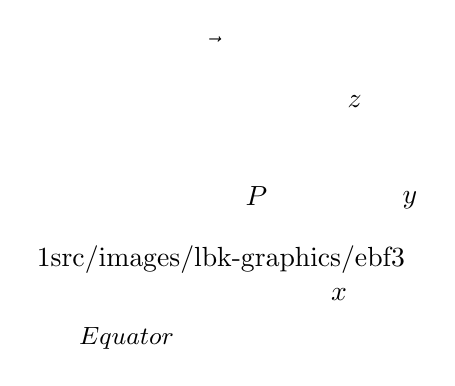
\begin{tikzpicture}
%   \draw[help lines,step=.5,lightgray] (-3,-3) grid (3,3) ;
%     \foreach \y in {-3,-2.5,...,3}
%     \draw (-3.2,\y) node[left]{\tiny\y} ;
%     \foreach \x in {-3,-2.5,...,3}
%     \draw (\x,3.2) node[above]{\tiny\x} ;
\node at% 
(0,0){\ingr{1}{src/images/lbk-graphics/ebf3}} ; 
   \node at(-.1,2.7) {$\vec{\gkw}$} ; 
    \node at(.75,2.4) {$\uvec{\gkw}$} ; 
    \node at(.45,.8) {$P$} ;
    \node at(2.4,.75) {$y$} ;
    \node at(1.7,2) {$z$} ;
    \node at(1.5,-.45) {$x$} ; 
    \node at(.28,.-.03) {$\gkl$} ; 
     \node at(-1.2,-1) {\small $\text{Equator}$} ; 
  \end{tikzpicture}
  \end{center}
\caption{Defining an earth-bound-frame at $P$}
\label{fig2.5}
\end{figure}
In what follows, we conveniently denote 
$\vec{w}_\sfx{\text{eff}}=(m\vec{g}+\vec{F}_t)$ and 
$\vec{g}_\sfx{\text{eff}}$ by $\pvec{w}$ and $\pvec{g}$ 
respectively. Then, Eqn.\eqref{nif.57} becomes
\begin{align}\label{nif.58}
m \vec{a}= \vec{w} +\vec{F}_a +\vec{F}_c.
\end{align}
Since $\vec{w}$ points vertically down at $P$, i.e., along 
the negative $z$-axis, we have
\begin{align}\label{nif.59}
\pvec{w} = (0,0,-mg').
\end{align}
Next, we calculate the Coriolis force $\vec{F}_c$ on $m$:
We get
\begin{align}\label{nif.60}
\vec{F}_c&=-2m\vec{\gkw} \times \vec{v}=
-2m\gkw
\begin{vmatrix}
 \eye & \jay & \kay \\
 -\cos\lambda& 0&\sin\lambda\\
 \dot{x} & \dot{y} & \dot{z}
\end{vmatrix}\notag
\\&=2m\gkw(\dot{y}\sin\lambda,\,-\dot{x}
\sin\lambda
-\dot{z}\cos\lambda,\,\dot{y}\cos\lambda).
\end{align}
Using Eqns.\eqref{nif.59}-\eqref{nif.60}, we may write
Eqn.\eqref{nif.58} in component-form as
\begin{align}\label{nif.61}
m\ddot{x} & =F_{ax}+2m\gkw\dot{y}\sin\lambda,\\
m\ddot{y} & =F_{ay}-2m\gkw(\dot{x}\sin\lambda
+\dot{z}\cos\lambda),\label{nif.62}\\
m\ddot{z} & =F_{az}-mg'+2m\gkw\dot{y}\cos\lambda,
\label{nif.63}
\end{align}
which are the equations of motion for a particle $m$ 
\index{equations of motion ! in an earth-bound frame} 
in the earth-bound-frame $S$ defined in \figref{fig2.5} 
at a place $P$ of latitude $\lambda$ at which the 
effective acceleration due to gravity is $g'$. These 
equations differ from the Newtonian equations with 
respect to a Galilei frame $S_1$ such as the one 
mentioned in the beginning paragraph of \S~2.9, if 
terms involving $\gkw\approx 
\num{7d-5}\,\si{rad.s^{-1}}$ can be neglected in 
comparison with components $F_{ax},F_{ay},F_{az}$ of 
the applied force.

\exm Find the maximal percent-decrease in the weight of an 
object due to the spin of the earth. 
\soln 
\begin{align} 
\frac{mR \gkw^2}{mg} = \frac{R \gkw^2}{g}&\approx\frac{6.4 
\times 10^6 \times (2\pi/86400)^2\; 
\SI{}{m.s^{-2}}}{10\;\SI{}{m.s^{-2}}} =0.003. 
\end{align} 
Therefore, the maximal percent-decrease in the weight of an 
object at the equator due to the spin of the earth is about 
0.3~.

\exm{Find the angle $\varepsilon $ between $\vec{g}$ and 
$\vec{g}_ {_ {\text{eff}}}$.} 

\soln Although exaggerated in \figref{fig2.6}, $\varepsilon 
$ is actually a very small angle. Since $m$ is at rest 
under the action of the three forces $m\vec{g}$, $\vec{T}$ 
and $(mr\gkw^2)\hat{\rho}$, we have, using the sine-rule of 
trigonometry, 
\begin{align}
\frac{mg}{\sin(\pi-\lambda-\varepsilon)}
=\frac{mg_\sfx{\text{eff}}}{\sin\lambda} =
\frac{mr\gkw^2}{\sin\varepsilon}.
\end{align}
%
\begin{figure}[H]
\begin{center}
\begin{tikzpicture}
%   \draw[help lines,step=.5,lightgray] (-3,-3) grid (3,3) ;
%     \foreach \y in {-3,-2.5,...,3}
%     \draw (-3.2,\y) node[left]{\tiny\y} ;
%     \foreach \x in {-3,-2.5,...,3}
%     \draw (\x,3.2) node[above]{\tiny\x} ;
%
\node at (0,0){\ingr{.8}{src/images/lbk-graphics/angle-g-geff}};
 \node at(2.1,-.2){$\vec{T}=m\vec{g}_{_{\nnt\text{eff}}}$}; 
 \node at(-.3,-2.7) {$mR\gkw^2\hat{\gkr}$} ; 
 \node at(-.6,-.2) {$m\vec{g}$} ; 
  \node at(1.25,1.5) {$\varepsilon$} ; 
  \node at(-1.25,-2.2) {$\gkl$} ; 
\end{tikzpicture}
\caption{}\label{fig2.6}
\end{center}
\end{figure}
%
So,
\begin{align}
\sin\varepsilon\approx \varepsilon =
(r\gkw^2/g_\sfx{\text{eff}}) \sin\lambda <
(r\gkw^2/g_\sfx{\text{eff}}) < (r\gkw^2/g),
\end{align}
as $ g_{\sfx{eff}}<g $. Using the numerical values $ 
g\approx$\SI{10}{m/s^2}, $r\sim \SI{6e6}{m}$ and 
$\gkw=2\pi/(24\times 60\times 60) \approx 
$\SI{.00007}{rad/s}, we get $\varepsilon 
\lesssim$\SI{0.003}{rad}$=10'$.

\vspace{-.3cm}

\subsection{Coriolis force on vertical motion}
\index{Coriolis force ! on vertical motion} Clearly, 
{vertical motion} corresponds to motion along the $z$-axis 
of the earth-bound frame defined above and in  such a 
motion we have $\dot{x}= \ddot{x}=\dot{y}= \ddot{y}=0, 
\dot{z}\neq 0$. From Eqn.\eqref{nif.60}, we get
\begin{align}
\vec{F}_{c}=2m\gkw(0, -\dot{z}\cos\gkl, 0).
\end{align}
for the Coriolis force on $m$ in vertical motion. Since, the
$y$-axis points east, and $-\dot{z} >0$ for a falling
particle, it follows that $F_{cx} =-2m\dot{z}\gkw$ is
positive. That is, {a falling particle `experiences' a 
Coriolis force due east}. Similarly, a rising particle 
experiences a Coriolis force due west.

\subsection{Coriolis force on horizontal motion}
\index{Coriolis force ! on horizontal motion} Horizontal 
motion in the chosen earth-bound frame corresponds to 
motion 
in the $x-y$ plane. Therefore, setting $\dot{z}=0 $ in 
Eqn.\eqref{nif.60}, we get the following expression for the 
Coriolis force on a particle of mass $m$:
\begin{align}\label{2.79x}
\vec{F}_{c}=2m\gkw(\dot{y}\sin\lambda,\,
-\dot{x}\sin\lambda,\,\dot{y}\cos\lambda).
\end{align}
Now, let us define the horizontal component 
$\vec{v}^\sfx{(h)}\equiv (\dot{x}\eye +\dot{y}\jay)$ of the 
velocity vector of the particle and the horizontal 
component 
$\vec{F}^\sfx{(h)}_c\equiv (F_{cx}\eye +F_{cy}\jay)$ of the 
Coriolis force on the particle. Then, we
observe that
\begin{align}
\vec{v}^\sfx{(h)}\dotp \vec{F}^\sfx{(h)}_c =
\dot{x}F_{cx}+\dot{y}F_{cy}=2m\gkw\sin\lambda\, (\dot {x}
\dot{y} -\dot{x}\dot{y})=0,
\end{align}
which shows that $\vec{F}^\sfx{(h)}_{c}$ is
at right angles to $\vec{v}^\sfx{(h)}$.

With reference to \figref{fig2.5}, suppose the particle is 
moving from south to north (i.e., towards the origin on the 
$x$-axis) at a place $P$ in the \textsl{northern 
hemisphere}. Then, the particle has $\dot{x}<0$. As 
$\gkp/2\geq\gkl\geq 0$ in the northern hemisphere, both 
$\cos\gkl$ and $\sin\gkl$ are positive so that from 
Eqn.\eqref{2.79x}), it follows that $F_\sfx{cy}>0$. 
Moreover, for this motion on the $x$-axis, we have 
$F_\sfx{cx}=0$ as $\dot{y}=0$. Thus, the particle 
experiences a Coriolis force $F_\sfx{cy}>0$ along the 
positive $y$-axis, i.e., \textsl{the particle is deflected 
due east which is to the right of the velocity 
$\vec{v}^\sfx{(h)}$ of the particle.}

On the other hand, if the particle is moving from north to 
south (i.e., away from the origin on the $x$-axis) at a 
place $P$ in the \textsl{northern hemisphere}, the particle 
has an $\dot{x}>0$, and, as before $\sin\gkl>0$ and 
$\dot{y}=0$ so that from Eqn.\eqref{2.79x}), we have 
$F_\sfx{cy}<0$. In other words, the particle experiences a 
Coriolis force $F_\sfx{cy}<0$ which is along the negative 
$y$-axis. As such, \textsl{the particle is deflected due 
west which is, again, to the right of the velocity 
$\vec{v}^\sfx{(h)}$ of the particle.}

We saw above, that the Coriolis force $\vec{F}_\sfx{c}$ 
causes moving objects on the surface of the earth to be 
deflected to the right (with respect to the direction of 
travel) in the northern hemisphere. Similarly, 
$\vec{F}_\sfx{c}$ causes moving objects on the surface of 
the earth to be deflected to the left in the southern 
hemisphere. It has been observed that the right-rails of 
railway-tracks on which trains move in the south-to-north 
direction are worn out more than the left-rails in the 
northern hemisphere.

One other large scale phenomemon that involves the Coriolis 
effect is the turn of the wind to the right in the Northern 
Hemisphere as happens in cyclones. We refer the the 
interested reader to the large amount of material available 
on this subject on the internet.

\vspace{-.4cm}
\subsection{The plumb line}
\index{plumb line}
Normally, we consider earth's gravitional force to act in 
the direction of a plumb line. We shall now examine to what 
extent the direction of a plumb line is affected by earth's 
rotation. In a Galilei frame in which the centre of sun is 
at rest, the earth has a translatory motion round the sun 
called {annual motion} and also a rotational motion about 
an 
axis passing through its centre called \textsl{diurnal 
motion}.

Consider a particle of mass $m$ at rest in the earth  
-bound 
frame $S$. We may maintain the mass $m$ in relative 
equilibrium in $S$, for example, by hanging it from a rigid 
support $A$ attached to the earth at $P$ by an inextensible 
mass-less string\footnote{In view of the large radius of 
the 
earth, the small separations between the points $P$, $m$  
and $A$ may be neglected compared to $R$ and we may assume 
that the the three points are essentially coincident}. 
\begin{figure}[H]
\begin{center}
\begin{tikzpicture}
%   \draw[help lines,step=.5,lightgray] (-3,-3) grid (3,3) ;
%     \foreach \y in {-3,-2.5,...,3}
%     \draw (-3.2,\y) node[left]{\tiny\y} ;
%     \foreach \x in {-3,-2.5,...,3}
%     \draw (\x,3.2) node[above]{\tiny\x} ;
%
\node at (0,0){\includegraphics[scale=1.6]% 
{src/images/lbk-graphics/plumb-line}};
 \node at(-1.1,-1.8) {$P$}; 
 \node at(.75,2.3) {$A$}; 
 \node at(1.15,1.2) {$\vec{T}$} ; 
 \node at(2.75,.1) {$\vec{F}_t$} ; 
  \node at(.1,.06) {$m$} ; 
  \node at(.8,-1.5) {$m\vec{g}$} ; 
    \node at(-1.95,-2.3) {\rm Earth} ; 
\end{tikzpicture}
\caption{Forces on a plumb-line}\label{fig2.7}
\end{center}
\end{figure}

% \fig{.9}{{lbk-graphics/plumb-line}}{Forces on a 
% plumb-line} 

Then, $A$ supports $m$ from falling by exerting a force 
$\vec{T}$ on $m$ which is conveyed (instantaneously) to $m$ 
through the connecting string. The force $\vec{T}$ is 
called 
the \index{tension in a string}{tension in the 
string}\footnote{If $\vec{T}$ is the `action' of $A$ on 
$m$, 
$m \vec{g}$ is the `reaction' of $m$ on $A$ and both these 
forces are conveyed through the string.}. Then, the forces 
that act on $m$ in the non-Galilei earth-bound frame $S$ 
are, (1) the gravitational pull $m\vec{g}$ of the earth, 
(2) 
the tension $\vec{T}$ in the string and (3) the transport 
force $\vec{F}_t $ that exists in the non-Galilei frame 
$S$. 
\begin{figure}[H]
\begin{center}
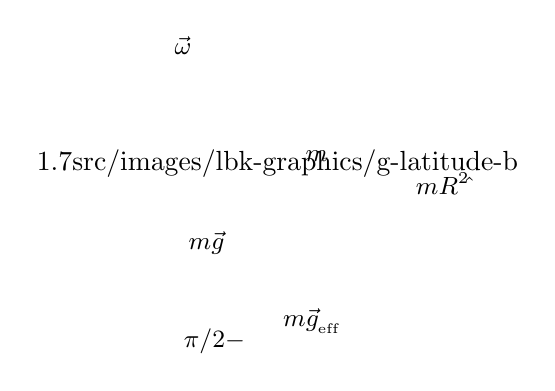
\begin{tikzpicture}
%   \draw[help lines,step=.5,lightgray] (-3,-3) grid (3,3) ;
%     \foreach \y in {-3,-2.5,...,3}
%     \draw (-3.0,\y) node[left]{\tiny\y} ;
%     \foreach \x in {-3,-2.5,...,3}
%     \draw (\x,3.0) node[above]{\tiny\x} ;
  \node at 
(0,0){\ingr{1.7}{src/images/lbk-graphics/g-latitude-b} };
 \node at(-1.2,1.5)  {\small $\vec{\omega}$} ;
 \node at(.5,0.1)  {\small $m$} ;
 \node at(2.1,-.25)  {\small $mR\gkw^2\hat{\gkr}$} ; 
 \node at(0.45,-2) {\small $m\vec{g}_{_{\rm{eff}}}$} ; 
 \node at(-.9,-1) {\small $m\vec{g}$} ; 
 \node at(-1.6,-1.6) {\small $\gkq$} ;  
 \node at(-.8,-2.25) {\small $\pi/2-\gkq$} ; 
\end{tikzpicture}
\caption{}\label{fig2.8}
\end{center}
\end{figure}

Let $m$ be at the \textsl{co-latitude} (\ie the {polar 
angle}) $\gkq$ on earth. Then $m$ is at a perpendicular 
distance of $R \sin\gkq$ from the spin-axis of the earth. 
($\lambda =\pi/2-\gkq$ is the {latitude} of $P$. See 
\figref{fig2.5}.) Since $m$ is at rest, the net force 
acting on it must be zero so that
 \begin{align} \vec{T}
=-\frac{GMm}{R^2}\,\hat{r} +(mR \gkw^2\sin
\gkq)\, \hat{\rho},
\end{align}
where $ (mR\gkw^2\,\sin\gkq) \, \hat{\rho}$ is the
centrifugal force on $m$ in the rotating earth-frame and
$what{\rho}$ is a unit vector perpendicular to the spin-axis
$\hat{z}$ of the earth.

If we define an \textsl{effective acceleration due to 
gravity at the place $P$} by $ T\equiv 
m\vec{g}_\sfx{\text{eff}}$, then 
the magnitude of $\vec{g}_\sfx{\text{eff}}$ is given by
\begin{align}\label{bg.17}
g^2_\sfx{\text{eff}}&=G^2M^2/R^4
-(2GM\gkw^2\,\sin\gkq) \, (\hat{r}
\dotp\hat{\rho})/R+R^2\gkw^4\,\sin^2
\gkq \notag\\
&=G^2M^2/R^4 -(2GM\gkw^2\,\sin^2\gkq)/R +R^2\gkw^4\,\sin^2 
\gkq \notag\\
&=G^2M^2/R^4+
[R^2\gkw^4-(2GM\gkw^2)/R]\sin^2 \gkq,
\end{align}
where we have written $\hat{r}
\dotp\hat{\rho}=\cos(\hat{r},\hat{\rho}
)=\cos\lambda=\sin\gkq $. 

\dfn The force $\vec{w}_\sfx{\text{eff}}\equiv 
m\vec{g}_\sfx{\text{eff}}$ is called the \textsl{effective 
weight} of $m$ at the place $P$.\index{effective 
weight}

\dfn The line-of-action of the effective weight at $P$ is
called the \textsl{vertical line} \index{vertical at a 
place} at $P$.

Therefore, the {effective weight} of $m$ at $P$, by 
definition, directed {vertically down} at $P$. At the 
equator, where $\gkq =90^\circ,\; \hat{r} =3\hat{\rho}$, 
$\vec{g}_\sfx{\text{eff}}$ has the {least value} given by
\begin{align}
g_\sfx{\text{eff}}&=\frac{GM}{R^2}-R \gkw^2 
=g-R \gkw^2.
\end{align}
At the poles ($(\gkq =0/\pi$ North/South),
$\vec{g}_\sfx{\text{eff}}$ has the {maximum value}
\begin{align}
g_\sfx{\text{eff}}=\frac{GM}{R^2}=g.
\end{align}
In between, $g_\sfx{\text{eff}}$ varies slightly with
co-latitude $\gkq$ as given by  Eqn.~\break\eqref{bg.17}.

\vspace{-.2cm}
\section{Larmor nutation}
\index{Larmor nutation} \index{Larmor theorem}


As an illustration of the methods of mechanics in an 
accelerated frame,  we discuss here the classical 
non-relativistic problem of the motion of a charged 
particle 
in an external central force field and a weak uniform 
magnetic field. We show that the motion of the kinetic 
angular momentum $\vec{L} = \vec{r}\times\vec{p}$ of the 
particle, in the so-called \textsl{Larmor approximation}, 
\index{Larmor approximation} is not a simple precession but 
is actually a composite motion involving precession as well 
as a high-frequency nutation. We analyse the 
precession-nutation motion of $\vec{L}$ in the Larmor 
approximation when the Larmor-frame-orbit (see \S2.12) of 
the charged particle is an ellipse (or a circle) in two 
cases, namely, the Coulomb-force and the Hooke-law-force, 
which are the only two central forces known to permit 
closed orbits. \index{closed orbits}

\hsl{Introduction}
It appears that only one exact solution is available for 
the 
classical non-relativistic problem of a  charged particle 
moving under the combined influence of an attractive 
central 
electric field and a uniform magnetic field. This special 
solution describes the circular orbit of a charged particle 
in a plane perpendicular to the applied uniform magnetic 
field. More general exact solutions for this problem do not 
exist although a variety of approximate solutions may be 
obtained through Larmor's theorem. Larmor's theorem as 
applied to this problem\footnote{R.P.Feynman, R.B.Leighton 
and M.Sands, \textsl{The Feynman Lectures on Phy -sics}, 
Reading, Massachusetts, Addison Wesley, 1964, 34-6--34-7. 
See also, (i) L.D.Landau and E.M.Lifshitz, 
\textsl{Mechanics}, Course of Theoretical Physics, Vol.~1, 
Pergamon Press, Oxford, 1976, pp 32--39, 70, and (ii) 
H.Goldstein, \textsl{Classical Mechanics}, Addison Wesley, 
London, 1980, pp 93, 107-109, 176-177, 233.} may  be 
stated as follows:
 
\hsl{Larmor theorem} Every bounded-orbit\footnote{A bound 
orbit is an orbit $\vec{r}=\vec{r}(t)$ in which $|\vec{r}|$ 
remains finite and non-zero.} of the charged particle 
moving 
in a Galilei frame under the action of the central force 
field and a sufficiently weak magnetic field is 
approximately a bounded orbit in the same central field, 
but 
without the magnetic field, when viewed from an appropriate 
rotating frame called the Larmor frame. \index{Larmor  
! frame}\index{Larmor  !  theorem}\index{Larmor  !  
frequency}

If we assume that the motion of the charged particle in 
such 
a precessing orbit generates a `pointlike magnetic 
dipole-moment whose magnitude is not affected by the motion 
it undergoes, then it follows that \footnote{H.Goldstein, 
\textsl{Classical Mechanics}, Addison Wesley, London, 1980, 
pp 93, 107-109, 176-177, 233.} the magnetic dipole 
precesses 
uniformly with the Larmor frequency\footnote{See 
Eqn.\eqref{eq:ln003} for a definition}. The assumption that 
the orbit is a pointlike magnetic moment is appropriate to 
permanent magnets or systems on an atomic or smaller scale 
and obviously is not valid for macroscopic charged particle 
orbits. Therefore, it is of some interest to study the 
motion of the magnetic moment $\vec{\mu}$ or the orbital 
angular momentum $\vec{L} = \vec{\mu}/{\gamma}$,  where 
$\gamma$ is the gyromagnetic ratio, in the case of 
macroscopic orbits.

Since a precessing charged particle orbit is essentially 
a `mag\-netic-top', we may expect the Larmor motion of 
$\vec{L}$ to involve nutation also in complete analogy 
with the problem of a massive top in a gravitational field. 
In fact, Landau and Lifshitz [8] show that in the case of a 
point charge executing bounded periodic motion under the 
influence of a central electrostatic field and a weak 
magnetic field, a suitably time-averaged motion of 
$\vec{L}$ 
is the familiar Larmor precession. Here, by restricting 
ourselves to a study of the motion of $\vec{L}$ in the 
Larmor approximation, we show that the detailed motion of 
$\vec{L}$ consists of a precession as well as a high 
frequency nutation. Obviously, we expect the second term on 
the right hand side of Eqn.\eqref{eq:ln002} to generate 
nutation-like features in the motion of 
$\vec{L}$\textsl{for 
macroscopic charged particle orbits} following 
Eqn.\eqref{eq:ln002} under the conditions of validity of 
the 
Larmor theorem.

\vspace{-.2cm}
\section{Motion of the angular momentum in the Larmor approximation}

The equation of motion of a negatively-charged 
particle\footnote{We have considered, here, specifically a 
particle of charge $-q$, obviously with the electron in 
mind. However, the discussion may be modified to cover the 
case of a positively charged particle by allowing $q$ to 
take positive values.} of char\-ge $-q < 0$ and mass $m$, 
moving in a Galilei frame under the combined influence of 
an external central force field $f(r)$ $\hat{r}$ and a 
uniform magnetic field $\vec{B}$ is given by 
\footnote{\textsl{Unlike elsewhere in this book where we 
employ the SI units, we work in the Gaussian CGS units in 
this discussion of Larmor motion.}}
\begin{align}
\dv{(m\vec{v})}{t} = f(r)\,{\hat{r}} -
(q/c){\vec{v}}\times{\vec{B}},
\label{eq:ln001}
\end{align}
where $\vec{r}$ is the position vector of the particle, 
$\hat{r}$ is a unit vector along $\vec{r}$, $\vec{v} = 
\dd\vec{r}/\dd t$ is the velocity of the particle and $c$ 
is 
the speed of light in vacuum. On cross-multiplying this 
equation by $\vec{r}$, we get
\begin{align}
\dv{\vec{L}}{t} =
-2m{\vec{r}}\times{({\vec{v}}\times{\vec{\gkw}})},
\label{eq:ln002}
\end{align}
where $\vec{L} = \vec{r}\times{m\vec{v}}$ is the kinetic
angular momentum of the particle,
\begin{align}
 \vec{\gkw} \equiv \frac{q\vec{B}}{2mc},
\label{eq:ln003}
\end{align}
and $\abs{\vec{\gkw}}$ is the `Larmor frequency'. Now, if 
we 
write the term $-2m{\vec{r}}\times{({\vec{v}}} 
\times{{\vec{\gkw}})}$ as the sum of two equal halves, 
express one of them using the Jacobi identity as \[ 
m{\vec{v}}\times{({\vec{\gkw}}\times{\vec{r}})} + 
m{\vec{\gkw}}\times{({\vec{r}}\times{\vec{v}})}, \] and add 
it 
to the other in equation (2.2), we obtain
\begin{align}
\dv{\vec{L}}{t} = {\vec{\gkw}}\times{\vec{L}} +
\dv{\vec{\Lambda}}{t},
\label{eq:ln004}
\end{align}
where we have defined
\begin{align}
 \vec{\Lambda} \equiv
m{\vec{r}}\times{({\vec{\gkw}}\times{\vec{r}})}.
\label{eq:ln005}
\end{align}
Although Eqn.\eqref{eq:ln002} and Eqn.\eqref{eq:ln004} are 
the 
same, the latter is more convenient in discussing the 
motion 
of $\vec{L}$. In fact Eqn.\eqref{eq:ln004} shows at once 
[10] 
that the motion of $\vec{L}$  would be a pure precession 
around $\vec{B}$ only when the second term 
$\dd\vec{\Lambda}/\dd t$ on the right hand side of 
Eqn.\eqref{eq:ln004} is either zero or is negligible in 
comparison with the first term 
${\vec{\gkw}}\times{\vec{L}}$. 
Since both these terms are of the same order in $\vec{B}$, 
it is clear that the motion of $\vec{L}$ can never be a 
simple precession however weak the magnetic field $\vec{B}$ 
may be.

The vector $\vec{\Lambda}$ above has a simple 
interpretation 
from the  standpoint of the so called Larmor frame, i.e., a 
reference frame which rotates with the angular velocity 
$\vec{\gkw}$ relative to the Galilei frame in which the 
problem is being studied. If we denote quantities referred 
to the Larmor frame by an asterisk (*) and the 
time-rates-of-change with respect to the Galilei and Larmor 
frames by $\dd{}/\dd t$ and $\dd{^*\!}/\dd t$ respectively, 
then we have [5] \[\dv{\vec{A}}{t} = \ldv{\bst}{\vec{A}}{t} 
+ {\vec{\gkw}}\times{\vec{A}}, \] which is a general 
relation valid for all vector functions $\vec{A}(t)$. Also, 
we assume that the origins of the two frames coincide, so 
that we have $\vec{r}(t) = \svec{r}(t)$ and this relation 
together with the fact that $\vec{\gkw}$ is a constant, 
leads to the following well-exploited relations for 
velocity 
and acceleration:
\begin{align}
& \vec{v} = \svec{v} + {\vec{\gkw}}\times{\vec{r}}; \;
   \vec{v} \equiv {\dd\vec{r}}/{\dd t}; \;
   \svec{v} \equiv {\dd^\bst\vec{r}}/{\dd t};
\label{eq:ln006}\\\notag
& \vec{a} = \svec{a} + 2{\vec{\gkw}}\times\svec{v}
+{\vec{\gkw}}\times{({\vec{\gkw}}}\times{\vec{r}});\notag\\
   &\vec{a} \equiv {\dd\vec{v}}/{\dd t};
\;\;\svec{a}\equiv \dd^\bst \svec{v}/{\dd t}.
\label{eq:ln007}
\end{align}
In the same manner, we obtain the following relation 
connecting kinetic angular momenta in the two frames of 
reference
\begin{align}
 \vec{L} = \svec{L}+ \vec{\Lambda}; ~
    \vec{L} \equiv {\vec{r}}\times{m\vec{v}};~
    \svec{L}\equiv {\vec{r}}\times{m\svec{v}}.
\label{eq:ln008}
\end{align}
This relation between angular momenta in the two  
frames, somehow, seems to have received little attention in 
the literature. The vector $\svec{L}$ in the above equation 
may be interpreted as the \textsl{angular momentum relative 
to the rotating frame} and the $\vec{\Lambda}$ as the 
angular momentum of transport. To appreciate the 
significance of $\vec{\Lambda}$ we may note that, for 
example, in the case of a rigid body, the vector $\svec{L}= 
{\sum{r}}\times \mbox{m} {\svec{v}}$ (where the summation 
extends over all the constituent particles) vanishes in the 
body rest frame and therefore the entire angular momentum 
appears as the transport angular momentum $\vec{\Lambda}$ 
in 
this frame.

On using Eqn.\eqref{eq:ln006}--Eqn.\eqref{eq:ln008}, 
Eqn.\eqref{eq:ln001} and Eqn.\eqref{eq:ln004}, we obtain
\begin{align}
m\svec{a}= m\ldv{\bst2}{\,\vec{r}}{t^{2}} =
f(r)\hat{r} +
 m{\vec{\gkw}}\times{({\vec{\gkw}}}\times{\vec{r})},
\label{eq:ln009}
\end{align}
and
\begin{align}
 \ldv{\bst}{\svec{L}}{t} ={\vec{\gkw}}\times{\vec{\Lambda}},
\label{eq:ln010}
\end{align}
which are exact equations corresponding to 
Eqn.\eqref{eq:ln001} and Eqn.\break \eqref{eq:ln002}, but written 
in the rotating Larmor frame. In the so-called Larmor 
approximation which corresponds to situations in which the 
magnetic field $\vec{B}$ is sufficiently weak and orbit of 
the particle is bounded in the sense described earlier, we 
neglect the second term on the right hand side of 
equation~Eqn.\eqref{eq:ln009} in comparison with the first 
and obtain
\begin{align}
 m\dv{^{*^{2}}\vec{r}}{t^{2}} \approx f(r)\,{\hat{r}},
\label{eq:ln011}
\end{align}
Taking the vector product of this equation with $\vec{r}$ 
then yields
\begin{align}
 \ldv{\bst}{\svec{L}}{t} \approx 0,
\label{eq:ln012}
\end{align}
which is the equation of motion of $\svec{L}$ in the Larmor 
approximation. Thus, in the Larmor approximation, 
$\svec{L}$ 
is a constant as viewed from the rotating frame, or, 
equivalently, it is a precessing vector satisfying
\begin{align}
 \ldv{\bst}{\svec{L}}{t} \approx
{\vec{\gkw}}\times{\svec{L}},
\label{eq:ln013}
\end{align}
as viewed from the Galilei (i.e., inertial) frame. It is 
gratifying to note that there is at least one angular 
momentum vector in the problem, namely $\svec{L}$, that 
executes a simple precessing motion in the Larmor 
approximation. However, it is $\vec{L}$, and not 
$\svec{L}$, 
which is the angular momentum of the particle in the 
Galilei 
frame and in view of Eqn.\eqref{eq:ln008}, the motion of 
$\vec{L}$ (in the Galilei frame) is more complex than a 
simple precession because $\vec{L}$ is the sum of a 
precessing vector $\svec{L}$ and the (moving) vector 
$\vec{\Lambda}$. In passing, we make an interesting 
observation on the canonical angular momentum $\vec{L}_{c} 
\equiv {\vec{r}}\times{(\vec{p} - q\vec{A}/{c})}$ of the 
charged particle in this problem. In a suitable gauge, the 
vector potential for a uniform magnetic field $\vec{B}$ may 
be written as $\vec{A} = -\vec{r}\times{B}/2$. With this 
$\vec{A}$, we obtain $\vec{L}_{c} = \vec{L} - \Lambda$. 
Comparing this with equation \eqref{eq:ln008} then shows 
that $\vec{L}_{c} = \svec{L}$. In view of this relation, 
Eqn.\eqref{eq:ln013} may also be interpreted as 
describing the Larmor precession of $\vec{L}_{c}$. Larmor's 
theorem in this form, for $\vec{L}_{c}$, may also be 
obtained directly without using the rotating frame [11]. 
Next, we wish to determine the motion of $\vec{L}$ in the 
Galilei frame. Before that, first, we mention very briefly 
about the only exact solution available for the equation 
\eqref{eq:ln001}. This solution describes the uniform 
circular  motion of a particle of charge $-q$ and mass $m$ 
in the Coulomb force field of a positive charge $q'$ at 
rest 
at the origin of coordinates of the Galilei frame. With $a$ 
denoting the radius of the circle and $\abs{\gkw}$ denoting 
the constant angular frequency, the solution mentioned is 
given by
\begin{align*}
\vec{r} = (a \cos\gkw' t, a \sin\gkw' t, 0), 
\end{align*} 
where
\vspace{-1\bsk}
\begin{align*}
\gkw' &\equiv \gkw \pm
\sqrt{\gkw_{0}^{2} + \gkw^{2}},\notag\\
\gkw 
&  = q \abs{\vec{B}}/2mc;\quad
\gkw_{0}= \sqrt{qq'/ma^{3}} > 0, 
\end{align*} 
and the $z$-axis of the Galilei frame has been chosen such 
that  $\vec{B} = (0, 0, B)$. A simple calculation then 
yields $\vec{L} = (0, 0, ma^2 \gkw')  = \text{constant}$. 
Leaving aside this exact solution which anyway has a 
constant $\vec{L}$ and is therefore not of interest to us, 
we consider approximate solutions of Eqn.\eqref{eq:ln001} 
obtained through the Larmor theorem. (In fact, our interest 
in these solutions is restricted to a study of the motion 
of 
the angular momenta rather than the orbits themselves.) We 
have a simple prescription for obtaining the orbital 
angular 
momentum vector associated with any such solution of 
Eqn.\eqref{eq:ln001} obtained through the Larmor theorem: 
First, we pick up an arbitrary bounded-orbit solution 
$\vec{r} = \vec{r}_{0}(t)$ of the problem \eqref{eq:ln011}. 
(It is important to note that $\vec{r}_{0}(t)$ so chosen is 
in fact an exact central force orbit and not an approximate 
one as required by equation Eqn.\eqref{eq:ln011}.) Then, 
using this vector $\vec{r}_{0}(t)$, we calculate vector 
field $\vec{\Lambda}(t)$ defined in 
equation~Eqn.\eqref{eq:ln005}. Next, we calculate the 
conserved orbital angular momentum vector  $\svec{L} = 
{\vec{r}_{0}} \times(m\,\dd{\vec{r}_{0}}/\dd t)$ of this 
orbit and use it to obtain the vector field $\vec{L} = 
\svec{L}+ \vec{\Lambda}$, which is the required orbital 
angular momentum in the Galilei frame (in the Larmor 
approximation).

We now use this prescription and calculate the $\vec{L}$ 
associated with an arbitrary, exact solution 
$\vec{r_{0}}(t)$ 
of Eqn.\eqref{eq:ln011}. Let $\vec{r_{0}}(t)$ 
expressed in the basis ($\eye,\jay, \kay$) of the Galilei 
frame be given by
\begin{align}
 \vec{r_{0}}(t) = x(t)\eye + y(t)\jay + z(t)\kay.
\label{eq:ln014}
\end{align}
Further, let the $z$-axis of the Galilei frame be chosen 
such that $\vec{B}$ is parallel or anti-parallel to $\kay$. 
Then
 \begin{align}
 \vec{\gkw} = \gkw\kay,
\label{eq:ln015}
\end{align}
where $\gkw > 0$ when $\vec{B}$ is parallel to $\kay$ and 
negative otherwise. Next, using equation 
Eqn.\eqref{eq:ln014}, Eqn.\eqref{eq:ln015} and definition 
Eqn.~\break\eqref{eq:ln005}, we obtain
\begin{align}
\vec{\Lambda} &=
m\vec{r}_0\times({\vec{\gkw}}\times{\vec{r}_{0}})
= -m\gkw \{ xz\eye + yz\jay- (x^2 + y^2)\kay \}.
\label{eq:ln016}
\end{align}
Since we know that $\svec{L}$ is a precessing vector as 
seen from the Galilei frame ($\eye, \jay, \kay$), and hence 
satisfies Eqn.\eqref{eq:ln013} (now exactly, as 
$\vec{r}_0 (t)$ is an exact solution of equation 
Eqn.\eqref{eq:ln011}), we may take it to be the general 
solution of Eqn.\eqref{eq:ln013} given below:
\begin{align}\label{eq:ln017}
\svec{L} = L_{0}(\sin\gkq \sin\varphi\,\eye - \sin\gkq
\cos\varphi\,\jay + \cos\gkq\,\kay).
\end{align}
Here $L_{0}$ and $\gkq$ are two constants of integration and
\begin{align}\label{eq:ln018}
 \varphi = \gkw t.
\end{align}
The angles $\gkq=$constant and $\varphi - \pi/2 = \gkw t 
-\pi/2$ are evidently the polar and azimuthal angles of 
$\svec{L}$ with respect to the Galilei frame ($\eye,\jay, 
\kay$) and these angles clearly show that the vector 
$\svec{L}$ precesses around the $z$-axis with angular 
frequency $\abs{\gkw}$. Now using equation 
Eqn.\eqref{eq:ln008}, Eqn.\eqref{eq:ln014} and 
Eqn.\eqref{eq:ln017}, we get $\vec{L}$ to the desired 
Larmor 
approximation as
\begin{align}
 \vec{L} = L_{x}\eye + L_{y}\jay + L_{z}\kay,
\label{eq:ln019}
\end{align}
where
\begin{align}
 L_{x} & = L_{0}\sin\gkq\, \sin\varphi - m \gkw x z,
\notag \\
 L_{y} & = -L_{0}\sin\gkq\, \cos\varphi - m \gkw y z,
\notag \\
 L_{z} & = L_{0}\cos\gkq + m\gkw(x^2 + y^2).
\label{eq:ln020}
\end{align}
These equations yield $\vec{L}$ once the central force 
orbit 
$\vec{r}_{0}(t)$ is specified as in equation 
Eqn.\eqref{eq:ln014}. This solves the problem in principle. 
However, in actual calculations it is  more convenient to 
specify the planar orbit $\vec{r}_{0}(t)$ in terms of two 
variables rather than in terms of the three variables $x, 
y, 
z$ as done above. We do this by introducing the rotating 
Larmor frame $(\hat{I}, \hat{J}, \hat{K})$ with 
corresponding coordinates, $X, Y, Z$, as follows. The plane 
of $\vec{r}_{0}(t)$ is taken to be the $X-Y$ plane so that 
$\svec{L}$ is always along the $Z$-axis. Further, we choose 
the $X$-axis to lie along the line of nodes formed by the 
$X-Y$ plane with the plane of the orbit $\vec{r}_{0}(t)$ as 
shown in figure~1. Then, constructing the rotation matrix 
connecting the two frames in terms of the Euler angles, we 
arrive at the coordinate transformation relating the two 
frames: 
\begin{align}
 &x = X\cos\varphi - Y\cos\gkq\,\sin\varphi, \notag\\
 & y = X\sin\varphi + Y\cos\gkq\,\cos\varphi,\notag\\
 & z = Y\sin\gkq.
\label{eq:ln021}
\end{align}
Substituting these in Eqn.Eqn.\eqref{eq:ln020}, we finally 
obtain the required formulae
\begin{align}
 &L_{x} = L_{0}\sin\gkq\,\sin\varphi - m\gkw
XY\sin\gkq\,\cos\varphi \notag \\
&\qquad +m\gkw Y^2\sin\gkq\,\cos\gkq\,\sin\varphi,
\notag \\
 & L_{y} = -L_{0}\sin\gkq\,\cos\varphi - m\gkw
XY\sin\gkq\,\sin\varphi \notag \\
&\qquad - m\gkw Y^2\sin\gkq\,\cos\gkq\,\cos\varphi,
\notag \\
 & L_{z} = L_{0}\cos\gkq + m\gkw X^2 + m\gkw
Y^2\cos^2\gkq.
\label{eq:ln022}
\end{align}
The components of $\vec{L}$ relative to the rotating frame  
$(\hat{I}, \hat{J}, \hat{K})$ are similarly found to be 
given by
 \begin{align}
 \vec{L}& = m\gkw\sin\gkq(-XY\,\hat{I} +
    X^2\,\hat{J})+ (L_{0} + m\gkw r_{0}^2\cos\gkq) \hat{K}.
\label{eq:ln023}
\end{align}
where $r_{0}^2 \equiv (X^2 + Y^2)$.

Before concluding this section, we restate the Larmor 
approximation in terms of a small dimensionless parameter. 
We may recall that for a bounded orbit $\vec{r} = 
\vec{r}(t), r \equiv \abs{\vec{r}}$ lies in the interval 
$0<r_{\min}\leq r \leq r_{\max} < \infty$. Now, let the 
magnitude of the central force $f(r)\,\hat{r}$ have its 
smallest value on the orbit, say, when $r = r_{1}$. Then, 
evidently, $\abs{f(r)\,\hat{r}} \geq \abs{f(r_{1})}$. We 
also note that 
$\abs{m{\vec{\gkw}}\times{({\vec{\gkw}}}\times{\vec{r}})} 
\leq m\gkw^2r_{\max}$. Thus, the Larmor approximation 
condition  
$\abs{f(r)} \gg \abs{m{\vec{\gkw}}\times{({\vec{\gkw}}} 
\times{\vec{r}})}$ may be expressed as
\begin{align}
 \abs{f(r_{1})} \gg m r_{\max}\,\gkw^2.
\label{eq:ln024}
\end{align}
If we now define the characteristic angular frequency
$\Omega>0$ associated with the bounded orbit of the
charged particle by
\begin{align}
 m\,{r}_{\max}\,\Omega^2 = \abs{f(r_{1})},
\label{eq:ln025}
\end{align}
the condition Eqn.\eqref{eq:ln024} reads
\begin{align}
 \Omega\gg \abs{\gkw}.
\label{eq:ln026}
\end{align}

\textsl{Thus, the Larmor approximation describes a 
situation 
in which the dimensionless parameter  $\abs{\gkw}/\Omega$ 
is 
`small'. }

Here we may note the fact that the modulus of $\gkw$ 
appears 
in equation  Eqn.\eqref{eq:ln026} above. This is so because 
$\gkw$, we may recall, can be positive as well as negative 
depending on whether $\vec{B}$ is parallel or anti-parallel 
to $\kay$. 

\vspace{-.2cm}

\section{Tracing the motion of {$\hat{L}$}}

\hsl{Elliptic Larmor frame orbits}Here, we trace the motion 
of the unit vector $\hat{L}$ in the case of such Galilei 
frame orbits $\vec{r}(t)$ for which the corresponding 
Larmor 
frame orbit $\vec{r_{0}}(t)$ is an ellipse. We know that 
(Bertrand's theorem: see Goldstein [4], or Landau and 
Lifshitz [1], p.32) the attractive inverse square law force 
and the Hooke law force (also called the space oscillator 
force) are the only two central forces which permit closed, 
and hence elliptic orbits. Hence our discussion would cover 
the cases of both these forces.

When $\hat{L}$ moves, its azimuth $\varphi_{L}$ and the 
polar angle $\gkq_{L}$ change with time. The angle 
$\varphi_{L}$ is given by $\tan \varphi_{L} = L_{y}/L_{x}$. 
On using Eqn.Eqn.\eqref{eq:ln022} and performing some  
elementary trigonometric rearrangement, we may invert this 
relation as,
\begin{align}
 \varphi_{L} = \varphi - (\pi/2) + \eta
    = \gkw t - (\pi/2) + \eta,
\label{eq:ln1}
\end{align}
where we have defined $\eta = \eta (t)$ by,
\begin{align}
 \tan \eta = -\frac{(m \gkw/{L_{0}}) XY}
    {\rule{0mm}{4mm}1 + \alpha Y^{2} \cos\gkq}\,.
\label{eq:ln2}
\end{align}
On the other hand, the polar angle $\gkq_{L}$ of $\hat{L}$
may be calculated from the relation,
\begin{align}
\cos \gkq_{L} = L_{z}/ |\vec{L}|.
\label{eq:ln3}
\end{align}
Now, if the Larmor frame orbit \{$ X(t), Y(t)$\} is 
specified, we may calculate the angles $\gkq_{L}$ and 
$\varphi_{L}$ as functions of time by using equations 
Eqn.\eqref{eq:ln1}, Eqn.\eqref{eq:ln2}, Eqn.\eqref{eq:ln3}. 
Then, the motion of $\hat{L}$ may be studied by considering 
the vector,
\begin{align}
 L_{\bot} \equiv \sin \gkq_{L} \cos \varphi_{L}\, \eye 
 + \sin \gkq_{L} \sin \varphi_{L} \, \jay, \label{eq:ln4}
\end{align}
which is the projection of $\hat{L}$ onto the $x-y$ plane
of the Galilei frame. The tip of this vector would trace a
circle if the motion of $\hat{L}$ is a pure precession.
Any non-circular tracing clearly indicates the presence of
nutation. This is as far as we can go with a general central
force field. Thus, we consider the two specific cases of
interest.

\hsl{Coulomb law elliptic orbits}
We begin by recalling some essential properties of an 
elliptic orbit [1] of a negatively-charged particle of 
charge $ -q<0 $ and mass $m$ moving in the Coulomb field of 
another positively particle of charge of charge $ q'>0 $ at 
rest at the coordinate origin (which also happens to be one 
of the two foci of the elliptic orbit). The parametric 
equations describing such an elliptic orbit are,
\begin{align}\label{eq:ln5}
X  &= a\,\rho; ~ Y = b\,\sigma; \quad 
\rho \equiv (\cos \xi - e);  
\quad \sigma \equiv \sin \xi; \notag \\
t&  = (T_{0}/2 \pi)(\xi - e \sin \xi), 
\end{align}
where $X = a\,\rho(t)$ and $Y = b\,\sigma(t)$ are the 
Cartesian coordinates of the particle tracing the ellipse. 
The constants $a, b$ and $e$ are respectively the semi-major 
axis, semi-minor axis and the eccentricity of the ellipse. 
The eccentric angle $\xi = \xi(t)$ increases by $2 \pi$ for 
one complete passage of the charged particle round the 
ellipse. The origin of time has been chosen such that $\xi = 
0$ at $t = 0$ and $\xi = 2 \pi$ at $t = T_{0}$, where 
$T_{0}$ is the period of the elliptic motion. The angular 
frequency $\gkw_{0}$ associated with $T_{0}$, is given by 
\begin{align*}
\gkw_{0} = 2 \pi/T_{0} = L_{0}/mab = 
\sqrt{-qq'/ma^{3}}, 
\end{align*}
where the positive constant $L_{0}$ is the magnitude of the 
conserved angular momentum associated with the elliptic 
orbit. Lastly, we note that the variables $\rho$ and 
$\sigma$ in Eqn.\eqref{eq:ln5} are dimensionless and have 
the respective  ranges $-(1+e) \leq \rho \leq (1-e)$ and $-1 
\leq \sigma \leq 1$.

Using Eqn.\eqref{eq:ln5}, Eqn.\eqref{eq:ln3}, and 
Eqn.\eqref{eq:ln022} we obtain the following equation:
\begin{small}
\begin{align}
&\nnnt\nnnt\nnnt\cos\gkq_{L} = \notag \\
    &\nnnt \nnnt \nnnt \frac{k + \varepsilon
\{(\frac{a}{b})\rho^{2} +
     (bk^{2}/a) \sigma^{2}\}}
     {\sqrt{1 + 2k \varepsilon \{(\frac{a}{b}) 
\rho^{2} +
(\frac{b}{a})\sigma^{2}\} +
     \varepsilon^{2} \{(\frac{a^{2}}{b^{2}})\rho^{4}
+ (1\nt + \nt k^{2}) 
(\frac{b^{2}k^{2}}{a^{2}})
    \nt+\nt \sigma^{4}\}}}\,.\notag\\
\label{eq:ln6}
\end{align}
\end{small} 
\nnt Here, in the above expression 
Eqn.\eqref{eq:ln6} for $\cos\gkq_{L}$, we have denoted 
$\cos\gkq$ by $k$ and have introduced the dimensionless 
parameter $\varepsilon \equiv \gkw/\gkw_{0}$. If we now 
observe that $\varepsilon$ and $\gkq$ are constants and the 
variables $\rho$ and $\sigma$ are periodic under $\xi 
\rightarrow \xi + 2\pi$ which corresponds to $t \rightarrow 
t + T_{0}$ (see remarks following Eqn.\eqref{eq:ln5}), it 
follows that $\cos \gkq_{L}$ given by Eqn.\eqref{eq:ln6} is 
a periodic function of time having the period $T_{0}$.
\begin{quote}
This means that in the Larmor approximation, $\vec{L}$ 
nutates with a time-period which is  precisely the 
orbital period $T_{0}$ of the charged particle in its 
elliptic Larmor frame orbit.
\end{quote}

\noindent Next, since the function $\eta(t)$ defined through 
Eqn.\eqref{eq:ln2} is also periodic under $t \rightarrow t + 
T_{0}$, we note that whenever $T \equiv 2 \pi /\abs{\gkw} = 
NT_{0}$, where $N$ is an integer, the azimuth $\varphi_{L}$ 
of $\vec{L}$ changes by $2\pi$ in a time $T$ during which 
$\gkq_{L}$, which has a time period $T_0 = T/N$, would go 
through exactly $N$ cycles. In other words, when $T = 
NT_{0}$, the tip of the unit vector $\hat{L}$ would trace a 
closed curve. When $\gkw$ and $\gkw_{0}$ are not 
commensurate, the tip of $\hat{L}$ does not trace a closed 
curve. In any case, the motion of $\hat{L}$ in the Larmor 
approximation is a composite motion involving both 
precession and nutation. The nutation frequency is given by 
$\gkw_{0}$ for elliptic paths of non-zero eccentricities. 
Interestingly, when $e$ becomes zero, i.e., when the Larmor 
frame orbit is a circle, the nutation frequency changes to 
2$\gkw_{0}$. This happens because, when $e = 0$, $\cos 
\gkq_{L}$ given by Eqn.\eqref{eq:ln6} becomes increasingly 
periodic; its period changes from $2\pi$ to $\pi$ for $\xi$ 
(or equivalently, $T_{0}$ to $T_{0}/2$ for $t$), as only 
even powers of $\rho$ and $\sigma$ appear in it. We also 
note that since the maximum separation $r_{\max}$ between 
$q'$ and $-q$ on the ellipse (equation Eqn.\eqref{eq:ln5}) 
is $a(1+e)$, the characteristic frequency $\vec{\Omega}$ of 
(Eqn.\eqref{eq:ln025} becomes $\vec{\Omega} = \gkw_{0}(1 + 
e)^{3/2}$. Thus the Larmor approximation condition (equation 
Eqn.\eqref{eq:ln026}) now requires $\gkw_{0} \gg 
(1+e)^{3/2}\abs{\gkw}$. As a consequence, the nutation 
frequencies ($\gkw_{0}$ or $2\gkw_{0}$) are very large 
compared to the Larmor frequency $\abs{\gkw}$.

An estimate of the magnitude of $\cos \gkq_{L}$, may be 
obtained as follows. We note that if we retain only terms of 
the order $O(\varepsilon)$ (in equation Eqn.\eqref{eq:ln6}), 
and substitute back for $\varepsilon$ as $\gkw/\gkw_{0}$, we 
obtain 
\begin{align*}
\cos \gkq_{L} = \cos \gkq + (\gkw a / \gkw_{0} b) 
\sin^{2}\gkq \rho^{2} + O(\varepsilon^{2}).        
\end{align*}
Incidentally, this formula shows that $\cos \gkq_{L} > \cos 
\gkq$ when $\gkw > 0 $ and $\cos \gkq_{L} < \cos \gkq $ when 
$\gkw < 0 $. Also, observing that $(\rho^{2})_{\max} = (1 + 
e)^2 $ and $(\rho^{2})_{\min} = 0$, we obtain
\begin{align}
& (\cos\gkq_L)_{\max} - (\cos \gkq)_{\min}  =
  \pm (\gkw a/ \gkw_{0}b)
  (1+e)^{2} \sin^{2} \gkq + o(\gkw^2)
\label{eq:ln7}
\end{align}
where the $+$ sign corresponds to $\gkw > 0$ and the $-$ 
sign to $\gkw < 0$. It is important to note that the leading 
term on the right hand side of (equation Eqn.\eqref{eq:ln7}) 
is linear in $\gkw$ and hence in the magnetic field strength 
$\abs{\vec{B}}$. Equation~Eqn.\eqref{eq:ln7}, however, does 
not yield an estimate of the nutation amplitude $\equiv 
(\gkq_{L})_{\max} - (\gkq)_{\min}$. It may be obtained 
numerically by calculating $\cos \gkq_{L}$ as a function of 
the angle $\xi$ and inverting.
\subsection{Model nutation graphs: Coulomb elliptic\\ orbits}
\begin{small}
Here, we draw some model precession-nutation  curves for 
the Coulomb case. These curves have been drawn by setting 
$L_{0} = 1, \gkw = \pm 1$ and $\gkq = \pi/4$. When $\gkq = 
\pi/4$, $\gkq_{L}$ also lies in (0, $\pi$/2) so that $\sin 
\gkq_{L}$ is positive. Therefore it may be calculated as 
$\sqrt{1-\cos^{2} \gkq_{L}}$ through equation 
Eqn.\eqref{eq:ln6}. The angle $\varphi_{L}$ has been 
calculated from equations Eqn.\eqref{eq:ln1} and 
Eqn.\eqref{eq:ln2}. 

Further, we have  chosen three convenient values for 
$\gkw_{0}$ namely $ 10,\break 100$ and $ 1000$ which yield closed 
nutation curves. In each of the following graphs
Figure 2.9, Figure 2.10 and Figure 2.11, the 
heavy-solid curve corresponds to $\gkw = 1$, the 
light-dashed one to $\gkw = -1$. The (solid) circle of 
radius $\sin \gkq = 1 / \sqrt{2}$ does not represent any 
real motion of $\vec{L}$, but has been drawn only for the 
sake of reference. (In fact, it is the circle $(\cos 
\gkq_{L})_{\min} = \cos \gkq = 1 / \sqrt{2}$ when $\gkw > 0$ 
and the circle $(\cos \gkq_{L})_{\max} = \cos \gkq = 1 / 
\sqrt{2}$ when $\gkw < 0 $).

The computed values of the nutation amplitude are as 
follows. For $\gkw = 1$, it is 36.4, 12.4 and 1.6 degrees, 
or, when $\gkw_{0}$ = 10, 100 and 1000 respectively. 
Similarly, for $\gkw = -1$, it is given by 122.8, 21.4 and 
1.6 degrees when $\gkw_{0}$ = 10, 100 and 1000 
respectively. These values clearly show that the nutation 
amplitude decreases as $\abs{\varepsilon}$ decreases. In 
fact, the precession slows down and the nutation dies out as 
$\abs{\varepsilon}$ decreases and eventually when 
$\abs{\varepsilon}$ touches zero, i.e., when $\vec{B} = 0$, 
$\vec{L}$ gets arrested at $\gkq_{L} = \gkq$ and 
$\varphi_{L} = -\pi/2$ (see equations Eqn.\eqref{eq:ln1}, 
Eqn.\eqref{eq:ln6} and the remarks following 
Eqn.\eqref{eq:ln018}).
\end{small}

\vspace{-.3cm}

\subsubsection*{Coulomb elliptic orbits: Model graph~1} 
\begin{figure}[H]
\centering
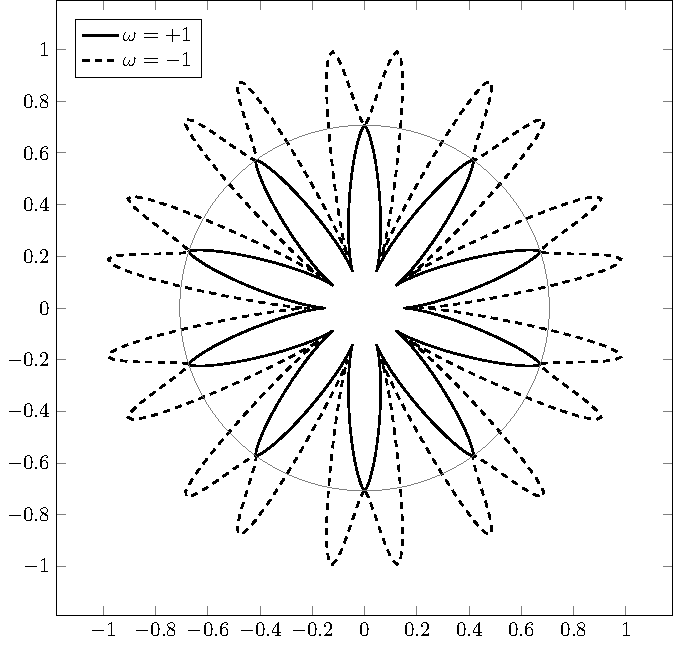
\includegraphics[scale=.4]{src/images/lbk-graphics/larm-c-10-1-45-1-10.pdf}
\caption*{Portrait of Galileo Galilei by Giusto Sustermans}\label{fig2.9}
\end{figure}
%~ \figl{.7}{lbk-graphics/larm-c-10-1-45-1-10.pdf}{}{fig2.9}

Type : Coulomb, $a= 10$, $b =1$, $\gkq = \ang{45}$, 
$\omega_0 = 10$, $t =0$ to $10$. The heavy-solid 
curve corresponds to $\gkw = 1$, the light-dashed curve to 
$\gkw = -1$. The (light solid) circle of radius $\sin \gkq 
= 1/\sqrt{2}$ does not represent any real motion of 
$\vec{L}$; it has been drawn only for the sake of reference.


\vspace{-.3cm}

\subsubsection*{Coulomb elliptic orbits: Model graph~2} 
\begin{figure}[H]
\centering
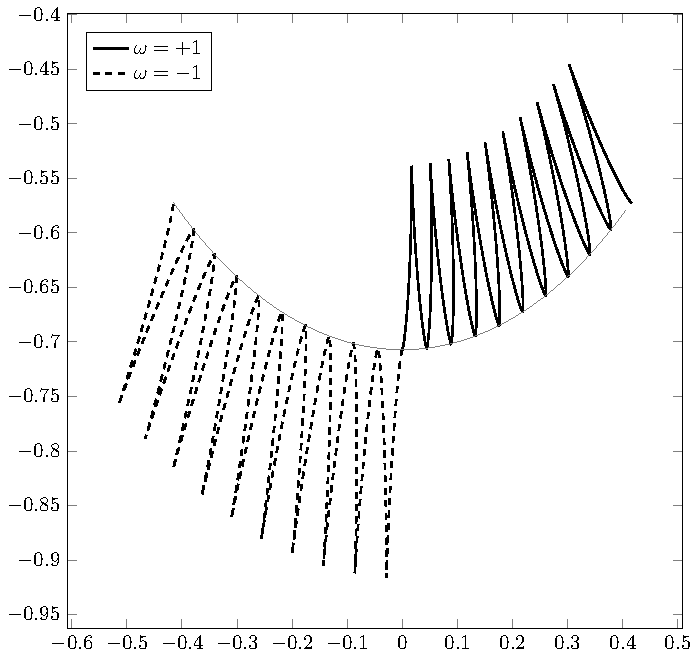
\includegraphics[scale=.4]{src/images/lbk-graphics/larm-c-10-1-45-1-100.pdf}
\caption*{}
\end{figure}
%~ \figl{.7}{lbk-graphics/larm-c-10-1-45-1-100.pdf}{}{fig2.10}

Type: Coulomb, $a = 10$, $b =1$, $\gkq = \ang{45}$, 
$\omega_0 = 100$, $t =0$ to $100$. The heavy-solid curve 
corresponds to $\gkw = 1$, the light-dashed curve to $\gkw = 
-1$. The (light solid) circle-segment has been drawn only 
for the sake of reference. 

\vspace{-.2cm}

\subsubsection*{Coulomb elliptic orbits: Model graph~3} 
\begin{figure}[H]
\centering
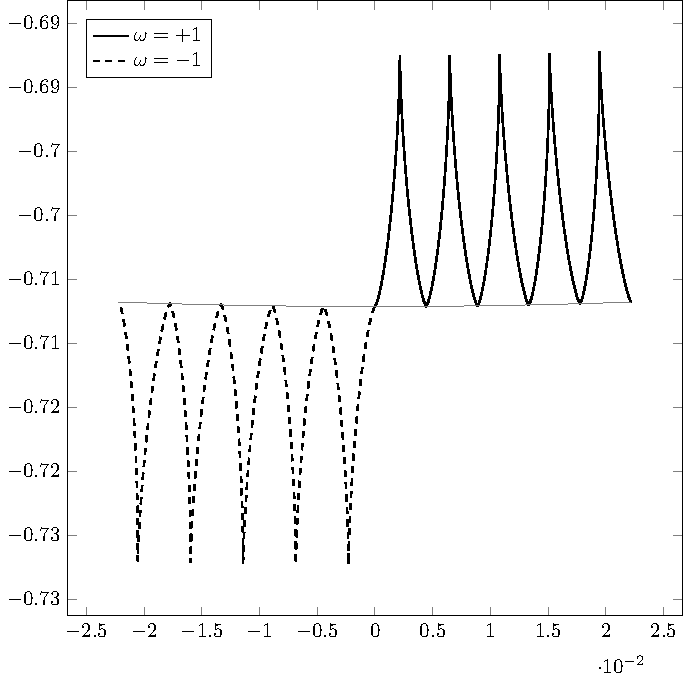
\includegraphics[scale=.5]{src/images/lbk-graphics/larm-c-10-1-45-1-1000.pdf}
\caption*{}
\end{figure}
%~ \figl{.7}{lbk-graphics/larm-c-10-1-45-1-1000.pdf}{}{fig2.11}

Type: Coulomb, $a = 10$, $b =1$, $\gkq = \ang{45}$, 
$\omega_0 = 1000$, $t=0$ to $1000$. The heavy-solid 
curve corresponds to $\gkw = 1$, the light-dashed curve to 
$\gkw = -1$. The (light solid) circle-segment of radius 
$\sin \gkq = 1 / \sqrt{2}$ has been drawn only for the sake 
of reference.

\subsection{Model nutation graphs: Hooke-law elliptic\\ orbits}
Writing the Hooke law central force as $f(r)\,\hat{r} = -m 
\gkw_{0}^{2} \vec{r}$, we obtain the following parametric 
equations to the elliptic orbit  (with the centre of 
attraction $\vec{r} = 0$ at the centre of the ellipse) [1], 
\begin{align}
 X &= a \cos\xi,\quad Y = b \cos(\xi + \delta), 
\text{and}\quad  \xi = \gkw_{0} t,
\label{eq:ln8}
\end{align}
where we have set $\xi = 0$ at $t = 0$. The other constant 
of integration $\delta$, when chosen appropriately, gives 
the various familiar Lissajous figures. We have specifically 
considered the case $\delta = -\pi/2$ which yields $X= 
a\cos\gkw t$ and $Y = b\sin\gkw t$ representing a central 
ellipse. 

Figure 2.12, Figure 2.13 and Figure fig2.14 
show some model precession nutation curves drawn with $a = 
10$ units and $b = 1$ unit. Further $\gkw_{0} = 10, 100 
\text{ and } 1000$\si{rad/s} respectively in 
Figure 2.12, Figure 2.13 and Figure 2.14. 

As with the Coulomb-graphs,  in each of the following 
Hook-law elliptic-orbit graphs, the heavy-solid curve 
corresponds to $\gkw = 1$, the light-dashed curve 
corresponds to $\gkw = -1$ whereas the (light-solid) circle 
of radius $\sin \gkq = 1 / \sqrt{2}$ has been drawn for the 
sake of reference. 

Lastly, we may note that the computed values of the nutation 
amplitudes in these graphs are as follows: For $\gkw = 1$, 
it is \ang{22.5}, \ang{3.8} and \ang{0.4} when $\gkw_{0} = 
10$, $100$ and $1000$ respectively. Similarly, for $\gkw = 
-1$, it is given by \ang{67.5}, \ang{4.4} and \ang{0.4} when 
$\gkw_{0} = 10$, $100$ and $1000$ \si{rad/s} respectively.

\subsubsection*{Hooke law elliptic orbits: Model graph~1} 
\begin{figure}[H]
\centering
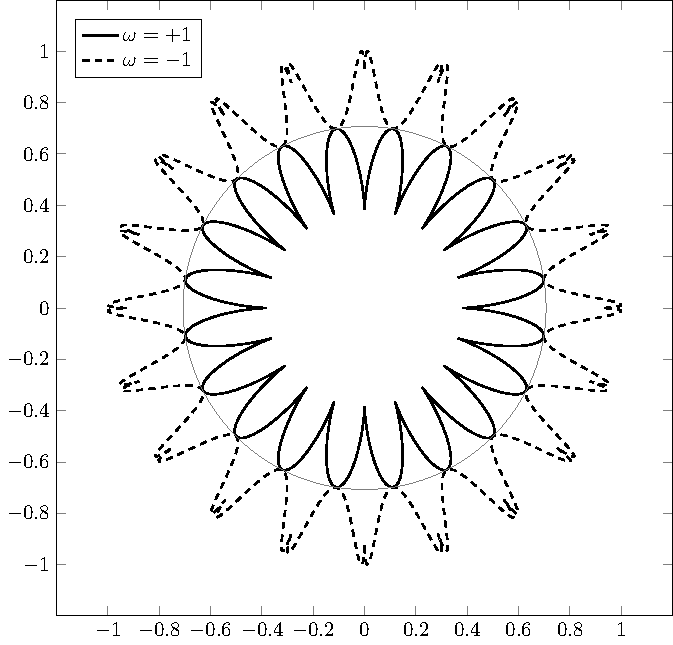
\includegraphics[scale=.5]{src/images/lbk-graphics/larm-h-10-1-45-1-10.pdf}
\caption*{}
\end{figure}
%~ \figl{.7}{lbk-graphics/larm-h-10-1-45-1-10.pdf}{}{fig2.12}

Type: Hooke, $a = 10 $, $b = 1$, $\gkq = \ang{45}$, 
$\omega_0 = 10$, $t=0$ to $10$. The heavy-solid 
curve corresponds to $\gkw = 1$ and the light-dashed curve 
corresponds to $\gkw = -1$. The (light-solid) circle of 
radius $\sin \gkq = 1 / \sqrt{2}$ has been drawn for the 
sake of reference.

\newpage

\subsubsection*{Hooke law elliptic orbits: Model graph~2} 
\begin{figure}[H]
\centering
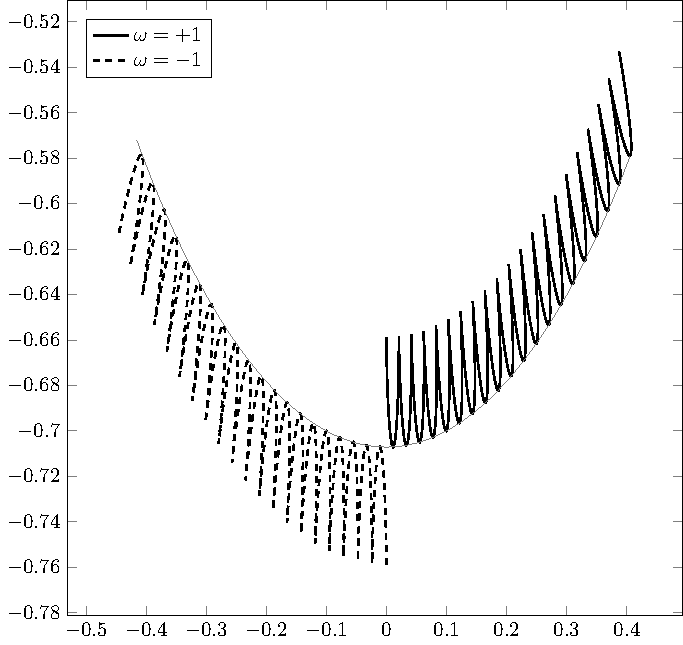
\includegraphics[scale=.4]{src/images/lbk-graphics/larm-h-10-1-45-1-100.pdf}
\caption*{}
\end{figure}
%~ \figl{.7}{lbk-graphics/larm-h-10-1-45-1-100.pdf}{}{fig2.13}

Type: Hooke, $a = 10 $, $b = 1$, $\gkq = \ang{45}$, 
$\omega_0 = 100$, $t=0$ to $100$.The heavy-solid curve 
corresponds to $\gkw = 1$ and the light-dashed curve 
corresponds to $\gkw = -1$. The light-solid curve, although 
does not look like it, is part of a circle of radius $\sin 
\gkq = 1 / \sqrt{2}$ and has been drawn for the sake of 
reference.

\subsubsection*{Hooke law elliptic orbits: Model graph~3}
\begin{figure}[H]
\centering
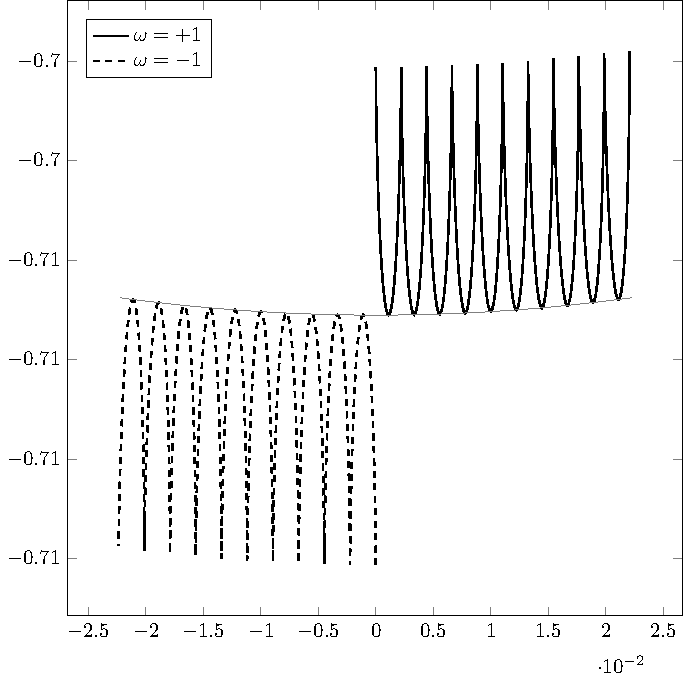
\includegraphics[scale=.4]{src/images/lbk-graphics/larm-h-10-1-45-1-1000.pdf}
\caption*{}
\vspace{-.3cm}
\end{figure}
%~ \figl{.7}{lbk-graphics/larm-h-10-1-45-1-1000.pdf}{}{fig2.14}

Type: Hooke, $a = 10 $, $b = 1$, $\gkq = \ang{45}$, 
$\omega_0 = 1000$, $t =0$ to $1000$. The heavy-solid curve 
corresponds to $\gkw = 1$ and the light-dashed curve 
corresponds to $\gkw = -1$. The light-solid curve is the 
segment of a  circle of radius $\sin \gkq = 1 / \sqrt{2}$ 
has been drawn for the sake of reference.

\newpage

\section*{Exercises}

\exise As a special case, show that when 
$\ddot{\vec{g}}(t)=0$, together with the given information 
that $\hat{g}$ is a constant, Eqn.\eqref{gt.4} reduces to a 
Galilei transformation (but with an unusual notation for the 
relative velocity !)

\exise The frame  $S':\{x',y',z'\}$ is 
generated by the non-Galilei transformation
\begin{align}
x'=x-\frac{1}{2}gt^2, \;
y'=y,\;z'=z,\quad g=\text{constant},
\end{align}
from a Galilei frame $S:\{x,  y, z\}$. By studying the 
motion of a point $(x'=\text{const}, 
y'=\text{const},z=\text{const}')$ which is permanently at 
rest in $S'$, prove that $S'$ advances with a uniform 
acceleration $\vec{g}=(g,0,0)$ relative to the `absolute 
frame' $S$.

\exise{Show that the following coordinate transformation 
defines a frame $S'$ which has a uniformly accelerated 
advancing motion relative to the absolute frame $S$.
\begin{align}\label{gt.3}
\pvec{r}&= \vec{r}-(1/2)\vec{a}\,t^2,
\quad \vec{a}
=\text{constant},\notag\\&\eye'=\eye,\;
\jay'=\jay,\;\kay'=\kay,
\end{align}}

\exise{Show that the following coordinate transformation 
yields a frame $S'$ which oscillates \index{frame ! 
oscillating} relative to the absolute frame:
\begin{align}\label{gt.8}
x'(t)&= x-\cos(\gkw t),\;y'=y,\;z'=z,\;
\gkw=\text{ constant},\notag \\
\eye'&=\eye,\; \jay'=\jay,\;\kay'=\kay.
\end{align}}

\exise{Find the forces that act on a particle which is in
relative equilibrium in a linearly accelerated frame.}


\begin{quote}
\begin{small}
\hsl{References}

[1] Stefan Banach, \textsl{Mechanics}, Translated by  
E J Scott, 1951, \textsl{Monografie Matematyczne}, 
   Warszawa (Poland).

[2] K N Srinivasa Rao, \textsl{Classical Mechanics},  
Universities Press, Hyderabad 500029, India,  Chapter~4.
\end{small}
\end{quote}

\newpage

\begin{quote}
\begin{small}


[1] \textsl{The Larmor Nutation}, K.N.Srinivasa Rao and 
A.V.Gopala Rao, Pramana--journal of Physics   (Indian
Academy of Sciences), {48},(1997), pp 755-788.

[2] \textsl{The geometry of Larmor Nutation},\\
K.N.Srinivasa Rao, A.V.Gopala Rao and A.R.Usha Devi, 
Pramana-journal of Physics (Indian  Academy of 
Sciences), 
{59}, (2002), pp 621-629. 
\end{small}
\end{quote}

